\documentclass[twoside]{book}

% Packages required by doxygen
\usepackage{fixltx2e}
\usepackage{calc}
\usepackage{doxygen}
\usepackage[export]{adjustbox} % also loads graphicx
\usepackage{graphicx}
\usepackage[utf8]{inputenc}
\usepackage{makeidx}
\usepackage{multicol}
\usepackage{multirow}
\PassOptionsToPackage{warn}{textcomp}
\usepackage{textcomp}
\usepackage[nointegrals]{wasysym}
\usepackage[table]{xcolor}

% Font selection
\usepackage[T1]{fontenc}
\usepackage[scaled=.90]{helvet}
\usepackage{courier}
\usepackage{amssymb}
\usepackage{sectsty}
\renewcommand{\familydefault}{\sfdefault}
\allsectionsfont{%
  \fontseries{bc}\selectfont%
  \color{darkgray}%
}
\renewcommand{\DoxyLabelFont}{%
  \fontseries{bc}\selectfont%
  \color{darkgray}%
}
\newcommand{\+}{\discretionary{\mbox{\scriptsize$\hookleftarrow$}}{}{}}

% Page & text layout
\usepackage{geometry}
\geometry{%
  a4paper,%
  top=2.5cm,%
  bottom=2.5cm,%
  left=2.5cm,%
  right=2.5cm%
}
\tolerance=750
\hfuzz=15pt
\hbadness=750
\setlength{\emergencystretch}{15pt}
\setlength{\parindent}{0cm}
\setlength{\parskip}{0.2cm}
\makeatletter
\renewcommand{\paragraph}{%
  \@startsection{paragraph}{4}{0ex}{-1.0ex}{1.0ex}{%
    \normalfont\normalsize\bfseries\SS@parafont%
  }%
}
\renewcommand{\subparagraph}{%
  \@startsection{subparagraph}{5}{0ex}{-1.0ex}{1.0ex}{%
    \normalfont\normalsize\bfseries\SS@subparafont%
  }%
}
\makeatother

% Headers & footers
\usepackage{fancyhdr}
\pagestyle{fancyplain}
\fancyhead[LE]{\fancyplain{}{\bfseries\thepage}}
\fancyhead[CE]{\fancyplain{}{}}
\fancyhead[RE]{\fancyplain{}{\bfseries\leftmark}}
\fancyhead[LO]{\fancyplain{}{\bfseries\rightmark}}
\fancyhead[CO]{\fancyplain{}{}}
\fancyhead[RO]{\fancyplain{}{\bfseries\thepage}}
\fancyfoot[LE]{\fancyplain{}{}}
\fancyfoot[CE]{\fancyplain{}{}}
\fancyfoot[RE]{\fancyplain{}{\bfseries\scriptsize Generated on Sun Feb 15 2015 09\+:37\+:39 for M\+M\+Reversi by Doxygen }}
\fancyfoot[LO]{\fancyplain{}{\bfseries\scriptsize Generated on Sun Feb 15 2015 09\+:37\+:39 for M\+M\+Reversi by Doxygen }}
\fancyfoot[CO]{\fancyplain{}{}}
\fancyfoot[RO]{\fancyplain{}{}}
\renewcommand{\footrulewidth}{0.4pt}
\renewcommand{\chaptermark}[1]{%
  \markboth{#1}{}%
}
\renewcommand{\sectionmark}[1]{%
  \markright{\thesection\ #1}%
}

% Indices & bibliography
\usepackage{natbib}
\usepackage[titles]{tocloft}
\setcounter{tocdepth}{3}
\setcounter{secnumdepth}{5}
\makeindex

% Hyperlinks (required, but should be loaded last)
\usepackage{ifpdf}
\ifpdf
  \usepackage[pdftex,pagebackref=true]{hyperref}
\else
  \usepackage[ps2pdf,pagebackref=true]{hyperref}
\fi
\hypersetup{%
  colorlinks=true,%
  linkcolor=blue,%
  citecolor=blue,%
  unicode%
}

% Custom commands
\newcommand{\clearemptydoublepage}{%
  \newpage{\pagestyle{empty}\cleardoublepage}%
}


%===== C O N T E N T S =====

\begin{document}

% Titlepage & ToC
\hypersetup{pageanchor=false,
             bookmarks=true,
             bookmarksnumbered=true,
             pdfencoding=unicode
            }
\pagenumbering{roman}
\begin{titlepage}
\vspace*{7cm}
\begin{center}%
{\Large M\+M\+Reversi \\[1ex]\large 1.\+0.\+0 }\\
\vspace*{1cm}
{\large Generated by Doxygen 1.8.9.1}\\
\vspace*{0.5cm}
{\small Sun Feb 15 2015 09:37:39}\\
\end{center}
\end{titlepage}
\clearemptydoublepage
\tableofcontents
\clearemptydoublepage
\pagenumbering{arabic}
\hypersetup{pageanchor=true}

%--- Begin generated contents ---
\chapter{Hierarchical Index}
\section{Class Hierarchy}
This inheritance list is sorted roughly, but not completely, alphabetically\+:\begin{DoxyCompactList}
\item \contentsline{section}{Board\+Position}{\pageref{struct_board_position}}{}
\item Q\+Dialog\begin{DoxyCompactList}
\item \contentsline{section}{Game\+Dialog}{\pageref{class_game_dialog}}{}
\item \contentsline{section}{Highscore}{\pageref{class_highscore}}{}
\item \contentsline{section}{Settings\+Dialog}{\pageref{class_settings_dialog}}{}
\end{DoxyCompactList}
\item Q\+Main\+Window\begin{DoxyCompactList}
\item \contentsline{section}{Main\+Window}{\pageref{class_main_window}}{}
\end{DoxyCompactList}
\item Q\+Object\begin{DoxyCompactList}
\item \contentsline{section}{Board}{\pageref{class_board}}{}
\item \contentsline{section}{Game}{\pageref{class_game}}{}
\item \contentsline{section}{Minimax}{\pageref{class_minimax}}{}
\end{DoxyCompactList}
\item Q\+Widget\begin{DoxyCompactList}
\item \contentsline{section}{Board\+Widget}{\pageref{class_board_widget}}{}
\end{DoxyCompactList}
\item \contentsline{section}{Settings\+Dialog\+:\+:Settings}{\pageref{struct_settings_dialog_1_1_settings}}{}
\item \contentsline{section}{Ui\+:\+:Settings}{\pageref{struct_ui_1_1_settings}}{}
\item \contentsline{section}{Test$<$ T $>$}{\pageref{class_test}}{}
\end{DoxyCompactList}

\chapter{Class Index}
\section{Class List}
Here are the classes, structs, unions and interfaces with brief descriptions\+:\begin{DoxyCompactList}
\item\contentsline{section}{\hyperlink{class_board}{Board} }{\pageref{class_board}}{}
\item\contentsline{section}{\hyperlink{struct_board_position}{Board\+Position} }{\pageref{struct_board_position}}{}
\item\contentsline{section}{\hyperlink{class_board_widget}{Board\+Widget} }{\pageref{class_board_widget}}{}
\item\contentsline{section}{\hyperlink{class_game}{Game} }{\pageref{class_game}}{}
\item\contentsline{section}{\hyperlink{class_game_dialog}{Game\+Dialog} }{\pageref{class_game_dialog}}{}
\item\contentsline{section}{\hyperlink{class_highscore}{Highscore} }{\pageref{class_highscore}}{}
\item\contentsline{section}{\hyperlink{class_main_window}{Main\+Window} }{\pageref{class_main_window}}{}
\item\contentsline{section}{\hyperlink{class_minimax}{Minimax} }{\pageref{class_minimax}}{}
\item\contentsline{section}{\hyperlink{struct_settings_dialog_1_1_settings}{Settings\+Dialog\+::\+Settings} }{\pageref{struct_settings_dialog_1_1_settings}}{}
\item\contentsline{section}{\hyperlink{struct_ui_1_1_settings}{Ui\+::\+Settings} }{\pageref{struct_ui_1_1_settings}}{}
\item\contentsline{section}{\hyperlink{class_settings_dialog}{Settings\+Dialog} }{\pageref{class_settings_dialog}}{}
\item\contentsline{section}{\hyperlink{class_test}{Test$<$ T $>$} }{\pageref{class_test}}{}
\end{DoxyCompactList}

\chapter{Class Documentation}
\hypertarget{class_board}{}\section{Board Class Reference}
\label{class_board}\index{Board@{Board}}
Inheritance diagram for Board\+:\begin{figure}[H]
\begin{center}
\leavevmode
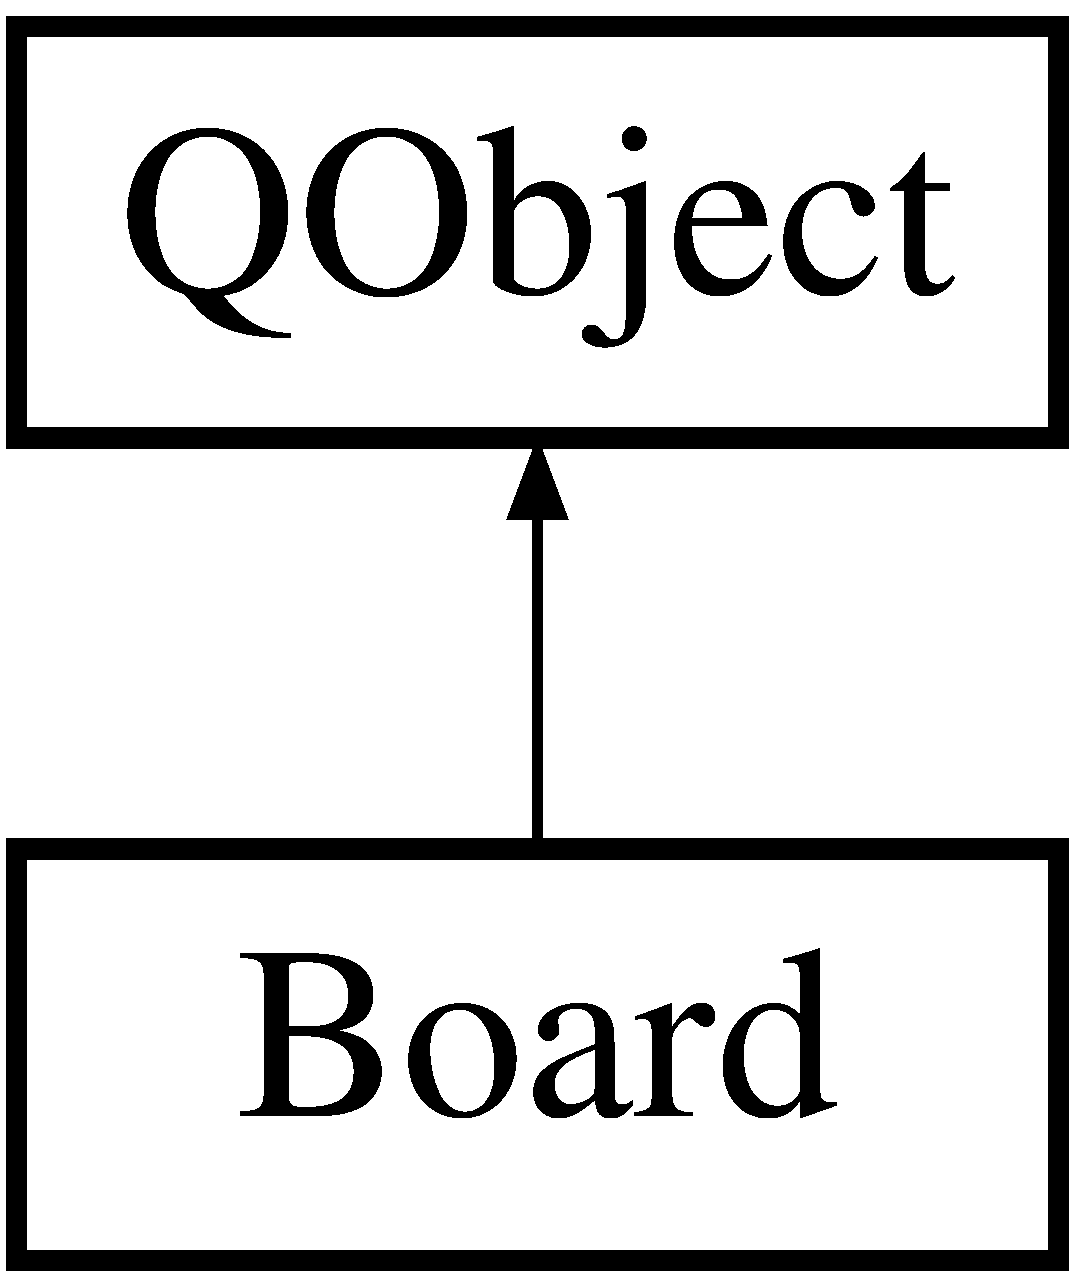
\includegraphics[height=2.000000cm]{class_board}
\end{center}
\end{figure}
\subsection*{Signals}
\begin{DoxyCompactItemize}
\item 
\hypertarget{class_board_a480fd8af3e8604d0568343dc2544903f}{}void {\bfseries board\+Changed} ()\label{class_board_a480fd8af3e8604d0568343dc2544903f}

\item 
\hypertarget{class_board_ae3a8556db5dcad7eb769f02c796b79d7}{}void {\bfseries move\+Made} (C\+E\+L\+L\+\_\+\+S\+T\+A\+T\+E player, C\+E\+L\+L\+\_\+\+S\+T\+A\+T\+E next\+Turn)\label{class_board_ae3a8556db5dcad7eb769f02c796b79d7}

\item 
\hypertarget{class_board_ad2a91234a1dfee298227dd8b10ce3446}{}void {\bfseries score\+Changed} (int white, int black)\label{class_board_ad2a91234a1dfee298227dd8b10ce3446}

\item 
\hypertarget{class_board_a7b96a501e83fe48ff825e73ad98fa929}{}void {\bfseries game\+Over} (C\+E\+L\+L\+\_\+\+S\+T\+A\+T\+E winner, int white, int black)\label{class_board_a7b96a501e83fe48ff825e73ad98fa929}

\item 
\hypertarget{class_board_a7cbf14fa69c5689b3dceeda86d3a15f5}{}void {\bfseries update\+Progress} (int value)\label{class_board_a7cbf14fa69c5689b3dceeda86d3a15f5}

\end{DoxyCompactItemize}
\subsection*{Public Member Functions}
\begin{DoxyCompactItemize}
\item 
\hyperlink{class_board_aedb1406901eb82feff01d9684ab4cb91}{Board} (int size=8, int style=1)
\item 
\hyperlink{class_board_a19e2c1f6c2baf8ab04cbd02f0cd2aebc}{Board} (const \hyperlink{class_board}{Board} \&)
\item 
\hyperlink{class_board_af73f45730119a1fd8f6670f53f959e68}{$\sim$\+Board} ()
\item 
int \hyperlink{class_board_a6f3891976ea2c25f4f8dc0080f977790}{get\+White\+Points} () const 
\item 
int \hyperlink{class_board_a47e7bc86cf4a514755b19d1afd3f0439}{get\+Black\+Points} () const 
\item 
int \hyperlink{class_board_ada12da9ad1391f41ba8dedd2facda89a}{get\+White\+Corner\+Points} () const 
\item 
int \hyperlink{class_board_a851b3f28fac5f40bf86520c79a81aef2}{get\+Black\+Corner\+Points} () const 
\item 
int \hyperlink{class_board_a298926d014849a98b85447783206eebc}{get\+White\+Edge\+Points} () const 
\item 
int \hyperlink{class_board_af3146d4d320bf5c6733dda2386635baf}{get\+Black\+Edge\+Points} () const 
\item 
int \hyperlink{class_board_a9c39cd47355ff518c21b94c0db920ecf}{get\+Score} () const 
\item 
Q\+List$<$ \hyperlink{struct_board_position}{Board\+Position} $>$ \hyperlink{class_board_a4831db9ba9cbc5bda9e60340c0483f04}{get\+Valid\+Moves} (C\+E\+L\+L\+\_\+\+S\+T\+A\+T\+E player) const 
\item 
bool \hyperlink{class_board_a52164c04edb93365f5bbada6e8ed2210}{is\+Valid\+Move} (\hyperlink{struct_board_position}{Board\+Position} pos, C\+E\+L\+L\+\_\+\+S\+T\+A\+T\+E player, Q\+List$<$ \hyperlink{struct_board_position}{Board\+Position} $>$ $\ast$flips=0) const 
\item 
bool \hyperlink{class_board_a3216c03487fee2408c8f3fd17c508dcc}{make\+Move} (\hyperlink{struct_board_position}{Board\+Position} pos, C\+E\+L\+L\+\_\+\+S\+T\+A\+T\+E player)
\item 
int \hyperlink{class_board_a94624883394858c34303952ac29af5fe}{get\+Board\+Size} () const 
\item 
int \hyperlink{class_board_a2da199b23725e0aa9ae4f9d9b0b477a3}{get\+Board\+Style} ()
\item 
bool \hyperlink{class_board_a4ba8975e38ece5b1665c004a480ae134}{is\+Cell\+Occupied} (\hyperlink{struct_board_position}{Board\+Position} pos) const 
\item 
C\+E\+L\+L\+\_\+\+S\+T\+A\+T\+E \hyperlink{class_board_a586374a43ddcc9444b93490072994bf1}{get\+Cell} (\hyperlink{struct_board_position}{Board\+Position} pos) const 
\item 
C\+E\+L\+L\+\_\+\+S\+T\+A\+T\+E \hyperlink{class_board_a2c6cfb671ca7cf610477d2495b8a227d}{get\+Who\+Is\+Next} () const 
\item 
C\+E\+L\+L\+\_\+\+S\+T\+A\+T\+E \hyperlink{class_board_aa670961269d7bee3128191635296b770}{get\+Enemy\+Of} (C\+E\+L\+L\+\_\+\+S\+T\+A\+T\+E) const 
\item 
bool \hyperlink{class_board_ab647ccf386b7a788ec8a1e19616abf88}{is\+Game\+Over} () const 
\item 
C\+E\+L\+L\+\_\+\+S\+T\+A\+T\+E \hyperlink{class_board_ae4d5573deabf4bc1052d4c4cfddf4a51}{get\+Winning\+Color} () const 
\item 
\hyperlink{struct_board_position}{Board\+Position} \hyperlink{class_board_a00f04a97d612c657b672867c034738f4}{get\+Best\+Move} () const 
\item 
\hyperlink{struct_board_position}{Board\+Position} \hyperlink{class_board_aae98cc0ea06e5dd9d96db347b96101b6}{get\+Last\+Move} () const 
\item 
void \hyperlink{class_board_adef66539dd52f84322525d2a4dfd2201}{calculate\+Best\+Move} (C\+E\+L\+L\+\_\+\+S\+T\+A\+T\+E player, int levels)
\end{DoxyCompactItemize}


\subsection{Constructor \& Destructor Documentation}
\hypertarget{class_board_aedb1406901eb82feff01d9684ab4cb91}{}\index{Board@{Board}!Board@{Board}}
\index{Board@{Board}!Board@{Board}}
\subsubsection[{Board}]{\setlength{\rightskip}{0pt plus 5cm}Board\+::\+Board (
\begin{DoxyParamCaption}
\item[{int}]{size = {\ttfamily 8}, }
\item[{int}]{style = {\ttfamily 1}}
\end{DoxyParamCaption}
)}\label{class_board_aedb1406901eb82feff01d9684ab4cb91}
Constructor style (0=default, 1=Future, 2=Super Mario)


\begin{DoxyParams}{Parameters}
{\em size} & \\
\hline
{\em style} & \\
\hline
\end{DoxyParams}
\hypertarget{class_board_a19e2c1f6c2baf8ab04cbd02f0cd2aebc}{}\index{Board@{Board}!Board@{Board}}
\index{Board@{Board}!Board@{Board}}
\subsubsection[{Board}]{\setlength{\rightskip}{0pt plus 5cm}Board\+::\+Board (
\begin{DoxyParamCaption}
\item[{const {\bf Board} \&}]{other}
\end{DoxyParamCaption}
)}\label{class_board_a19e2c1f6c2baf8ab04cbd02f0cd2aebc}
Copy constructor


\begin{DoxyParams}{Parameters}
{\em other} & \\
\hline
\end{DoxyParams}
\hypertarget{class_board_af73f45730119a1fd8f6670f53f959e68}{}\index{Board@{Board}!````~Board@{$\sim$\+Board}}
\index{````~Board@{$\sim$\+Board}!Board@{Board}}
\subsubsection[{$\sim$\+Board}]{\setlength{\rightskip}{0pt plus 5cm}Board\+::$\sim$\+Board (
\begin{DoxyParamCaption}
{}
\end{DoxyParamCaption}
)}\label{class_board_af73f45730119a1fd8f6670f53f959e68}
Destructor 

\subsection{Member Function Documentation}
\hypertarget{class_board_adef66539dd52f84322525d2a4dfd2201}{}\index{Board@{Board}!calculate\+Best\+Move@{calculate\+Best\+Move}}
\index{calculate\+Best\+Move@{calculate\+Best\+Move}!Board@{Board}}
\subsubsection[{calculate\+Best\+Move}]{\setlength{\rightskip}{0pt plus 5cm}void Board\+::calculate\+Best\+Move (
\begin{DoxyParamCaption}
\item[{C\+E\+L\+L\+\_\+\+S\+T\+A\+T\+E}]{player, }
\item[{int}]{difficulty}
\end{DoxyParamCaption}
)}\label{class_board_adef66539dd52f84322525d2a4dfd2201}
Calculates best move by using minimax algorithm for a specific player and ai difficulty


\begin{DoxyParams}{Parameters}
{\em player} & \\
\hline
{\em difficulty} & \\
\hline
\end{DoxyParams}
\hypertarget{class_board_a00f04a97d612c657b672867c034738f4}{}\index{Board@{Board}!get\+Best\+Move@{get\+Best\+Move}}
\index{get\+Best\+Move@{get\+Best\+Move}!Board@{Board}}
\subsubsection[{get\+Best\+Move}]{\setlength{\rightskip}{0pt plus 5cm}{\bf Board\+Position} Board\+::get\+Best\+Move (
\begin{DoxyParamCaption}
{}
\end{DoxyParamCaption}
) const}\label{class_board_a00f04a97d612c657b672867c034738f4}
A getter for the actual calculated best move

\begin{DoxyReturn}{Returns}
\hyperlink{struct_board_position}{Board\+Position} 
\end{DoxyReturn}
\hypertarget{class_board_a851b3f28fac5f40bf86520c79a81aef2}{}\index{Board@{Board}!get\+Black\+Corner\+Points@{get\+Black\+Corner\+Points}}
\index{get\+Black\+Corner\+Points@{get\+Black\+Corner\+Points}!Board@{Board}}
\subsubsection[{get\+Black\+Corner\+Points}]{\setlength{\rightskip}{0pt plus 5cm}int Board\+::get\+Black\+Corner\+Points (
\begin{DoxyParamCaption}
{}
\end{DoxyParamCaption}
) const}\label{class_board_a851b3f28fac5f40bf86520c79a81aef2}
Get points of B\+L\+A\+C\+K corner count

\begin{DoxyReturn}{Returns}
int 
\end{DoxyReturn}
\hypertarget{class_board_af3146d4d320bf5c6733dda2386635baf}{}\index{Board@{Board}!get\+Black\+Edge\+Points@{get\+Black\+Edge\+Points}}
\index{get\+Black\+Edge\+Points@{get\+Black\+Edge\+Points}!Board@{Board}}
\subsubsection[{get\+Black\+Edge\+Points}]{\setlength{\rightskip}{0pt plus 5cm}int Board\+::get\+Black\+Edge\+Points (
\begin{DoxyParamCaption}
{}
\end{DoxyParamCaption}
) const}\label{class_board_af3146d4d320bf5c6733dda2386635baf}
Get points of B\+L\+A\+C\+K edge count

\begin{DoxyReturn}{Returns}
int 
\end{DoxyReturn}
\hypertarget{class_board_a47e7bc86cf4a514755b19d1afd3f0439}{}\index{Board@{Board}!get\+Black\+Points@{get\+Black\+Points}}
\index{get\+Black\+Points@{get\+Black\+Points}!Board@{Board}}
\subsubsection[{get\+Black\+Points}]{\setlength{\rightskip}{0pt plus 5cm}int Board\+::get\+Black\+Points (
\begin{DoxyParamCaption}
{}
\end{DoxyParamCaption}
) const}\label{class_board_a47e7bc86cf4a514755b19d1afd3f0439}
Get point of B\+L\+A\+C\+K player

\begin{DoxyReturn}{Returns}
int 
\end{DoxyReturn}
\hypertarget{class_board_a94624883394858c34303952ac29af5fe}{}\index{Board@{Board}!get\+Board\+Size@{get\+Board\+Size}}
\index{get\+Board\+Size@{get\+Board\+Size}!Board@{Board}}
\subsubsection[{get\+Board\+Size}]{\setlength{\rightskip}{0pt plus 5cm}int Board\+::get\+Board\+Size (
\begin{DoxyParamCaption}
{}
\end{DoxyParamCaption}
) const}\label{class_board_a94624883394858c34303952ac29af5fe}
Get board size dimension

\begin{DoxyReturn}{Returns}
int 
\end{DoxyReturn}
\hypertarget{class_board_a2da199b23725e0aa9ae4f9d9b0b477a3}{}\index{Board@{Board}!get\+Board\+Style@{get\+Board\+Style}}
\index{get\+Board\+Style@{get\+Board\+Style}!Board@{Board}}
\subsubsection[{get\+Board\+Style}]{\setlength{\rightskip}{0pt plus 5cm}int Board\+::get\+Board\+Style (
\begin{DoxyParamCaption}
{}
\end{DoxyParamCaption}
)}\label{class_board_a2da199b23725e0aa9ae4f9d9b0b477a3}
Get board style (0=Default, 1=Future, 2=Super Mario)

\begin{DoxyReturn}{Returns}
int 
\end{DoxyReturn}
\hypertarget{class_board_a586374a43ddcc9444b93490072994bf1}{}\index{Board@{Board}!get\+Cell@{get\+Cell}}
\index{get\+Cell@{get\+Cell}!Board@{Board}}
\subsubsection[{get\+Cell}]{\setlength{\rightskip}{0pt plus 5cm}C\+E\+L\+L\+\_\+\+S\+T\+A\+T\+E Board\+::get\+Cell (
\begin{DoxyParamCaption}
\item[{{\bf Board\+Position}}]{position}
\end{DoxyParamCaption}
) const}\label{class_board_a586374a43ddcc9444b93490072994bf1}
Get the C\+E\+L\+L\+\_\+\+S\+T\+A\+T\+E (0=E\+M\+P\+T\+Y, 1=W\+H\+I\+T\+E, 2=B\+L\+A\+C\+K) at a specific position


\begin{DoxyParams}{Parameters}
{\em position} & \\
\hline
\end{DoxyParams}
\begin{DoxyReturn}{Returns}
C\+E\+L\+L\+\_\+\+S\+T\+A\+T\+E 
\end{DoxyReturn}
\hypertarget{class_board_aa670961269d7bee3128191635296b770}{}\index{Board@{Board}!get\+Enemy\+Of@{get\+Enemy\+Of}}
\index{get\+Enemy\+Of@{get\+Enemy\+Of}!Board@{Board}}
\subsubsection[{get\+Enemy\+Of}]{\setlength{\rightskip}{0pt plus 5cm}C\+E\+L\+L\+\_\+\+S\+T\+A\+T\+E Board\+::get\+Enemy\+Of (
\begin{DoxyParamCaption}
\item[{C\+E\+L\+L\+\_\+\+S\+T\+A\+T\+E}]{color}
\end{DoxyParamCaption}
) const}\label{class_board_aa670961269d7bee3128191635296b770}
Get\textquotesingle{}s the enemey of a player Need this for valid move and make\+Move methods


\begin{DoxyParams}{Parameters}
{\em color} & \\
\hline
\end{DoxyParams}
\begin{DoxyReturn}{Returns}
C\+E\+L\+L\+\_\+\+S\+T\+A\+T\+E 
\end{DoxyReturn}
\hypertarget{class_board_aae98cc0ea06e5dd9d96db347b96101b6}{}\index{Board@{Board}!get\+Last\+Move@{get\+Last\+Move}}
\index{get\+Last\+Move@{get\+Last\+Move}!Board@{Board}}
\subsubsection[{get\+Last\+Move}]{\setlength{\rightskip}{0pt plus 5cm}{\bf Board\+Position} Board\+::get\+Last\+Move (
\begin{DoxyParamCaption}
{}
\end{DoxyParamCaption}
) const}\label{class_board_aae98cc0ea06e5dd9d96db347b96101b6}
A getter for the last made move

\begin{DoxyReturn}{Returns}
\hyperlink{struct_board_position}{Board\+Position} 
\end{DoxyReturn}
\hypertarget{class_board_a9c39cd47355ff518c21b94c0db920ecf}{}\index{Board@{Board}!get\+Score@{get\+Score}}
\index{get\+Score@{get\+Score}!Board@{Board}}
\subsubsection[{get\+Score}]{\setlength{\rightskip}{0pt plus 5cm}int Board\+::get\+Score (
\begin{DoxyParamCaption}
{}
\end{DoxyParamCaption}
) const}\label{class_board_a9c39cd47355ff518c21b94c0db920ecf}
Get overall score, calculated from edge, base and corner count Was meant to be used in highscore view

\begin{DoxyReturn}{Returns}
int 
\end{DoxyReturn}
\hypertarget{class_board_a4831db9ba9cbc5bda9e60340c0483f04}{}\index{Board@{Board}!get\+Valid\+Moves@{get\+Valid\+Moves}}
\index{get\+Valid\+Moves@{get\+Valid\+Moves}!Board@{Board}}
\subsubsection[{get\+Valid\+Moves}]{\setlength{\rightskip}{0pt plus 5cm}Q\+List$<$ {\bf Board\+Position} $>$ Board\+::get\+Valid\+Moves (
\begin{DoxyParamCaption}
\item[{C\+E\+L\+L\+\_\+\+S\+T\+A\+T\+E}]{player}
\end{DoxyParamCaption}
) const}\label{class_board_a4831db9ba9cbc5bda9e60340c0483f04}
Get a list of valid moves by player


\begin{DoxyParams}{Parameters}
{\em player} & \\
\hline
\end{DoxyParams}
\begin{DoxyReturn}{Returns}
Q\+List$<$\+Board\+Position$>$ 
\end{DoxyReturn}
\hypertarget{class_board_ada12da9ad1391f41ba8dedd2facda89a}{}\index{Board@{Board}!get\+White\+Corner\+Points@{get\+White\+Corner\+Points}}
\index{get\+White\+Corner\+Points@{get\+White\+Corner\+Points}!Board@{Board}}
\subsubsection[{get\+White\+Corner\+Points}]{\setlength{\rightskip}{0pt plus 5cm}int Board\+::get\+White\+Corner\+Points (
\begin{DoxyParamCaption}
{}
\end{DoxyParamCaption}
) const}\label{class_board_ada12da9ad1391f41ba8dedd2facda89a}
Get points of W\+H\+I\+T\+E corner count

\begin{DoxyReturn}{Returns}
int 
\end{DoxyReturn}
\hypertarget{class_board_a298926d014849a98b85447783206eebc}{}\index{Board@{Board}!get\+White\+Edge\+Points@{get\+White\+Edge\+Points}}
\index{get\+White\+Edge\+Points@{get\+White\+Edge\+Points}!Board@{Board}}
\subsubsection[{get\+White\+Edge\+Points}]{\setlength{\rightskip}{0pt plus 5cm}int Board\+::get\+White\+Edge\+Points (
\begin{DoxyParamCaption}
{}
\end{DoxyParamCaption}
) const}\label{class_board_a298926d014849a98b85447783206eebc}
Get points of W\+H\+I\+T\+E edge count

\begin{DoxyReturn}{Returns}
int 
\end{DoxyReturn}
\hypertarget{class_board_a6f3891976ea2c25f4f8dc0080f977790}{}\index{Board@{Board}!get\+White\+Points@{get\+White\+Points}}
\index{get\+White\+Points@{get\+White\+Points}!Board@{Board}}
\subsubsection[{get\+White\+Points}]{\setlength{\rightskip}{0pt plus 5cm}int Board\+::get\+White\+Points (
\begin{DoxyParamCaption}
{}
\end{DoxyParamCaption}
) const}\label{class_board_a6f3891976ea2c25f4f8dc0080f977790}
Get point of W\+H\+I\+T\+E player

\begin{DoxyReturn}{Returns}
int 
\end{DoxyReturn}
\hypertarget{class_board_a2c6cfb671ca7cf610477d2495b8a227d}{}\index{Board@{Board}!get\+Who\+Is\+Next@{get\+Who\+Is\+Next}}
\index{get\+Who\+Is\+Next@{get\+Who\+Is\+Next}!Board@{Board}}
\subsubsection[{get\+Who\+Is\+Next}]{\setlength{\rightskip}{0pt plus 5cm}C\+E\+L\+L\+\_\+\+S\+T\+A\+T\+E Board\+::get\+Who\+Is\+Next (
\begin{DoxyParamCaption}
{}
\end{DoxyParamCaption}
) const}\label{class_board_a2c6cfb671ca7cf610477d2495b8a227d}
Get who\textquotesingle{}s turn is next

\begin{DoxyReturn}{Returns}
C\+E\+L\+L\+\_\+\+S\+T\+A\+T\+E 
\end{DoxyReturn}
\hypertarget{class_board_ae4d5573deabf4bc1052d4c4cfddf4a51}{}\index{Board@{Board}!get\+Winning\+Color@{get\+Winning\+Color}}
\index{get\+Winning\+Color@{get\+Winning\+Color}!Board@{Board}}
\subsubsection[{get\+Winning\+Color}]{\setlength{\rightskip}{0pt plus 5cm}C\+E\+L\+L\+\_\+\+S\+T\+A\+T\+E Board\+::get\+Winning\+Color (
\begin{DoxyParamCaption}
{}
\end{DoxyParamCaption}
) const}\label{class_board_ae4d5573deabf4bc1052d4c4cfddf4a51}
Who won?

\begin{DoxyReturn}{Returns}
C\+E\+L\+L\+\_\+\+S\+T\+A\+T\+E 
\end{DoxyReturn}
\hypertarget{class_board_a4ba8975e38ece5b1665c004a480ae134}{}\index{Board@{Board}!is\+Cell\+Occupied@{is\+Cell\+Occupied}}
\index{is\+Cell\+Occupied@{is\+Cell\+Occupied}!Board@{Board}}
\subsubsection[{is\+Cell\+Occupied}]{\setlength{\rightskip}{0pt plus 5cm}bool Board\+::is\+Cell\+Occupied (
\begin{DoxyParamCaption}
\item[{{\bf Board\+Position}}]{position}
\end{DoxyParamCaption}
) const}\label{class_board_a4ba8975e38ece5b1665c004a480ae134}
Checks if cell is occupied by a player at a specific position


\begin{DoxyParams}{Parameters}
{\em position} & \\
\hline
\end{DoxyParams}
\begin{DoxyReturn}{Returns}
bool 
\end{DoxyReturn}
\hypertarget{class_board_ab647ccf386b7a788ec8a1e19616abf88}{}\index{Board@{Board}!is\+Game\+Over@{is\+Game\+Over}}
\index{is\+Game\+Over@{is\+Game\+Over}!Board@{Board}}
\subsubsection[{is\+Game\+Over}]{\setlength{\rightskip}{0pt plus 5cm}bool Board\+::is\+Game\+Over (
\begin{DoxyParamCaption}
{}
\end{DoxyParamCaption}
) const}\label{class_board_ab647ccf386b7a788ec8a1e19616abf88}
Is the game over?

\begin{DoxyReturn}{Returns}
bool 
\end{DoxyReturn}
\hypertarget{class_board_a52164c04edb93365f5bbada6e8ed2210}{}\index{Board@{Board}!is\+Valid\+Move@{is\+Valid\+Move}}
\index{is\+Valid\+Move@{is\+Valid\+Move}!Board@{Board}}
\subsubsection[{is\+Valid\+Move}]{\setlength{\rightskip}{0pt plus 5cm}bool Board\+::is\+Valid\+Move (
\begin{DoxyParamCaption}
\item[{{\bf Board\+Position}}]{position, }
\item[{C\+E\+L\+L\+\_\+\+S\+T\+A\+T\+E}]{player, }
\item[{Q\+List$<$ {\bf Board\+Position} $>$ $\ast$}]{flips = {\ttfamily 0}}
\end{DoxyParamCaption}
) const}\label{class_board_a52164c04edb93365f5bbada6e8ed2210}
Checks if the move at a specific position by an specific player is valid


\begin{DoxyParams}{Parameters}
{\em position} & \\
\hline
{\em player} & \\
\hline
{\em flips} & \\
\hline
\end{DoxyParams}
\begin{DoxyReturn}{Returns}
bool 
\end{DoxyReturn}
\hypertarget{class_board_a3216c03487fee2408c8f3fd17c508dcc}{}\index{Board@{Board}!make\+Move@{make\+Move}}
\index{make\+Move@{make\+Move}!Board@{Board}}
\subsubsection[{make\+Move}]{\setlength{\rightskip}{0pt plus 5cm}bool Board\+::make\+Move (
\begin{DoxyParamCaption}
\item[{{\bf Board\+Position}}]{position, }
\item[{C\+E\+L\+L\+\_\+\+S\+T\+A\+T\+E}]{player}
\end{DoxyParamCaption}
)}\label{class_board_a3216c03487fee2408c8f3fd17c508dcc}
Does a move to a specific position by player


\begin{DoxyParams}{Parameters}
{\em position} & \\
\hline
{\em player} & \\
\hline
\end{DoxyParams}
\begin{DoxyReturn}{Returns}
bool 
\end{DoxyReturn}


The documentation for this class was generated from the following files\+:\begin{DoxyCompactItemize}
\item 
board.\+h\item 
board.\+cpp\end{DoxyCompactItemize}

\hypertarget{struct_board_position}{}\section{Board\+Position Struct Reference}
\label{struct_board_position}\index{Board\+Position@{Board\+Position}}
\subsection*{Public Attributes}
\begin{DoxyCompactItemize}
\item 
\hypertarget{struct_board_position_adfc976b5c3c1387ac6f03a618bd0d8bb}{}int {\bfseries x}\label{struct_board_position_adfc976b5c3c1387ac6f03a618bd0d8bb}

\item 
\hypertarget{struct_board_position_a99e9b7bc5d0061dfafb23d07baa5e3db}{}int {\bfseries y}\label{struct_board_position_a99e9b7bc5d0061dfafb23d07baa5e3db}

\end{DoxyCompactItemize}


The documentation for this struct was generated from the following file\+:\begin{DoxyCompactItemize}
\item 
board.\+h\end{DoxyCompactItemize}

\hypertarget{class_board_widget}{}\section{Board\+Widget Class Reference}
\label{class_board_widget}\index{Board\+Widget@{Board\+Widget}}
Inheritance diagram for Board\+Widget\+:\begin{figure}[H]
\begin{center}
\leavevmode
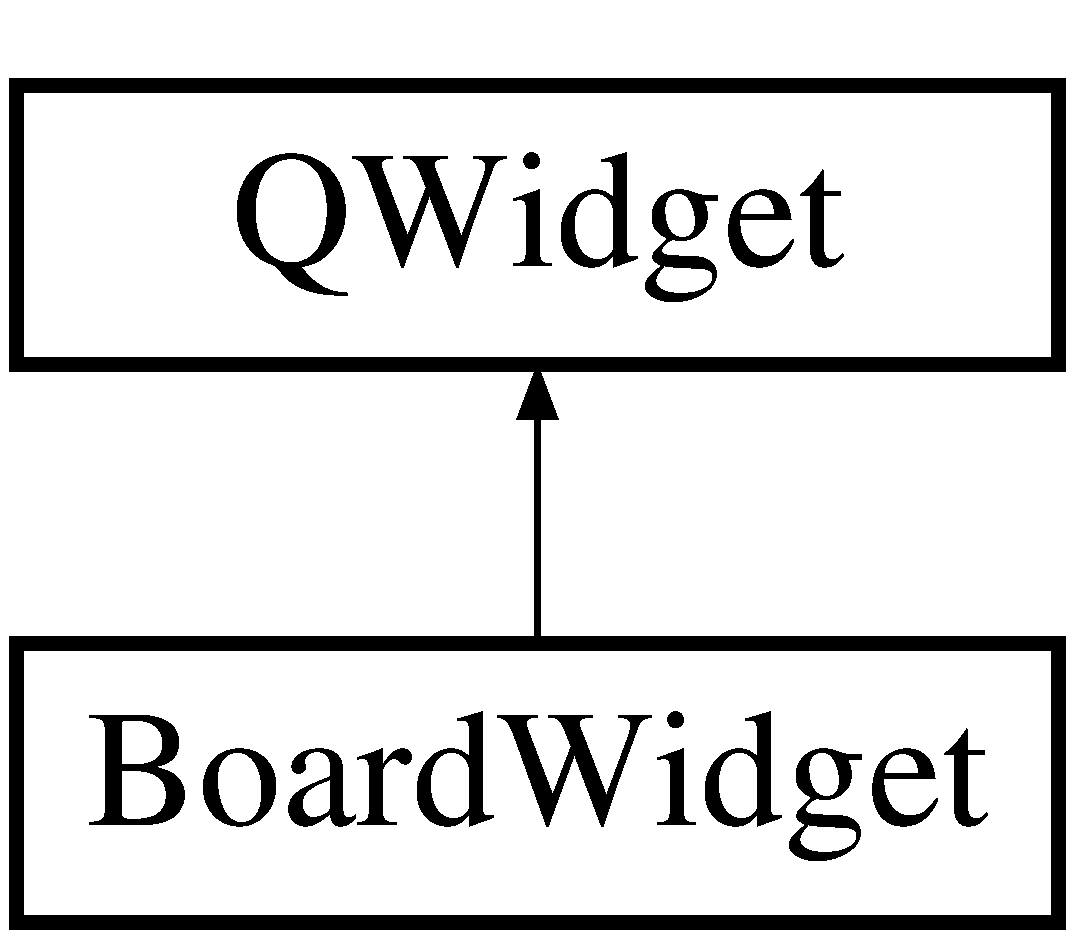
\includegraphics[height=2.000000cm]{class_board_widget}
\end{center}
\end{figure}
\subsection*{Signals}
\begin{DoxyCompactItemize}
\item 
\hypertarget{class_board_widget_adba731e80188fa0e43e925978997d2ce}{}void {\bfseries cell\+Clicked} (const \hyperlink{struct_board_position}{Board\+Position} cell)\label{class_board_widget_adba731e80188fa0e43e925978997d2ce}

\end{DoxyCompactItemize}
\subsection*{Public Member Functions}
\begin{DoxyCompactItemize}
\item 
\hyperlink{class_board_widget_a260ca35e417d25cc3e27401825793140}{Board\+Widget} (Q\+Shared\+Pointer$<$ \hyperlink{class_board}{Board} $>$ board, Q\+Widget $\ast$parent=0)
\item 
\hyperlink{class_board_widget_a532acccc2b203b2418e2b0bc358d7886}{Board\+Widget} (Q\+Widget $\ast$parent=0)
\item 
Q\+Size \hyperlink{class_board_widget_a86fa804cef03ad6ba2ee9f7b7b5323eb}{size\+Hint} () const 
\item 
void \hyperlink{class_board_widget_a0e0b3f9a57f30fd7aa13fab160cc91c1}{set\+Board} (Q\+Shared\+Pointer$<$ \hyperlink{class_board}{Board} $>$ board)
\item 
Q\+Shared\+Pointer$<$ \hyperlink{class_board}{Board} $>$ \hyperlink{class_board_widget_a34253aacadef1560220ead326bfc469d}{get\+Board} () const 
\end{DoxyCompactItemize}
\subsection*{Protected Member Functions}
\begin{DoxyCompactItemize}
\item 
void \hyperlink{class_board_widget_a634c28449979224320c787c771e5f1e5}{paint\+Event} (Q\+Paint\+Event $\ast$)
\item 
void \hyperlink{class_board_widget_afd5248764d8f9e334060870e676b41e7}{mouse\+Release\+Event} (Q\+Mouse\+Event $\ast$)
\item 
void \hyperlink{class_board_widget_a8c5fec911b5c86c37f5adba5f1be9aec}{mouse\+Press\+Event} (Q\+Mouse\+Event $\ast$)
\end{DoxyCompactItemize}


\subsection{Constructor \& Destructor Documentation}
\hypertarget{class_board_widget_a260ca35e417d25cc3e27401825793140}{}\index{Board\+Widget@{Board\+Widget}!Board\+Widget@{Board\+Widget}}
\index{Board\+Widget@{Board\+Widget}!Board\+Widget@{Board\+Widget}}
\subsubsection[{Board\+Widget}]{\setlength{\rightskip}{0pt plus 5cm}Board\+Widget\+::\+Board\+Widget (
\begin{DoxyParamCaption}
\item[{Q\+Shared\+Pointer$<$ {\bf Board} $>$}]{board, }
\item[{Q\+Widget $\ast$}]{parent = {\ttfamily 0}}
\end{DoxyParamCaption}
)\hspace{0.3cm}{\ttfamily [explicit]}}\label{class_board_widget_a260ca35e417d25cc3e27401825793140}
Constructor


\begin{DoxyParams}{Parameters}
{\em board} & \\
\hline
{\em parent} & \\
\hline
\end{DoxyParams}
\hypertarget{class_board_widget_a532acccc2b203b2418e2b0bc358d7886}{}\index{Board\+Widget@{Board\+Widget}!Board\+Widget@{Board\+Widget}}
\index{Board\+Widget@{Board\+Widget}!Board\+Widget@{Board\+Widget}}
\subsubsection[{Board\+Widget}]{\setlength{\rightskip}{0pt plus 5cm}Board\+Widget\+::\+Board\+Widget (
\begin{DoxyParamCaption}
\item[{Q\+Widget $\ast$}]{parent = {\ttfamily 0}}
\end{DoxyParamCaption}
)}\label{class_board_widget_a532acccc2b203b2418e2b0bc358d7886}
Constructor with no board initialized


\begin{DoxyParams}{Parameters}
{\em parent} & \\
\hline
\end{DoxyParams}


\subsection{Member Function Documentation}
\hypertarget{class_board_widget_a34253aacadef1560220ead326bfc469d}{}\index{Board\+Widget@{Board\+Widget}!get\+Board@{get\+Board}}
\index{get\+Board@{get\+Board}!Board\+Widget@{Board\+Widget}}
\subsubsection[{get\+Board}]{\setlength{\rightskip}{0pt plus 5cm}Q\+Shared\+Pointer$<$ {\bf Board} $>$ Board\+Widget\+::get\+Board (
\begin{DoxyParamCaption}
{}
\end{DoxyParamCaption}
) const}\label{class_board_widget_a34253aacadef1560220ead326bfc469d}
Get the actual board

\begin{DoxyReturn}{Returns}
Q\+Shared\+Pointer$<$\+Board$>$ 
\end{DoxyReturn}
\hypertarget{class_board_widget_a8c5fec911b5c86c37f5adba5f1be9aec}{}\index{Board\+Widget@{Board\+Widget}!mouse\+Press\+Event@{mouse\+Press\+Event}}
\index{mouse\+Press\+Event@{mouse\+Press\+Event}!Board\+Widget@{Board\+Widget}}
\subsubsection[{mouse\+Press\+Event}]{\setlength{\rightskip}{0pt plus 5cm}void Board\+Widget\+::mouse\+Press\+Event (
\begin{DoxyParamCaption}
\item[{Q\+Mouse\+Event $\ast$}]{event}
\end{DoxyParamCaption}
)\hspace{0.3cm}{\ttfamily [protected]}}\label{class_board_widget_a8c5fec911b5c86c37f5adba5f1be9aec}
Is needed to prevent mouse spam behaviour in mouse\+Release\+Event


\begin{DoxyParams}{Parameters}
{\em event} & \\
\hline
\end{DoxyParams}
\hypertarget{class_board_widget_afd5248764d8f9e334060870e676b41e7}{}\index{Board\+Widget@{Board\+Widget}!mouse\+Release\+Event@{mouse\+Release\+Event}}
\index{mouse\+Release\+Event@{mouse\+Release\+Event}!Board\+Widget@{Board\+Widget}}
\subsubsection[{mouse\+Release\+Event}]{\setlength{\rightskip}{0pt plus 5cm}void Board\+Widget\+::mouse\+Release\+Event (
\begin{DoxyParamCaption}
\item[{Q\+Mouse\+Event $\ast$}]{event}
\end{DoxyParamCaption}
)\hspace{0.3cm}{\ttfamily [protected]}}\label{class_board_widget_afd5248764d8f9e334060870e676b41e7}
Calls cell clicked event when mouse is released above a cell


\begin{DoxyParams}{Parameters}
{\em event} & \\
\hline
\end{DoxyParams}
\hypertarget{class_board_widget_a634c28449979224320c787c771e5f1e5}{}\index{Board\+Widget@{Board\+Widget}!paint\+Event@{paint\+Event}}
\index{paint\+Event@{paint\+Event}!Board\+Widget@{Board\+Widget}}
\subsubsection[{paint\+Event}]{\setlength{\rightskip}{0pt plus 5cm}void Board\+Widget\+::paint\+Event (
\begin{DoxyParamCaption}
\item[{Q\+Paint\+Event $\ast$}]{}
\end{DoxyParamCaption}
)\hspace{0.3cm}{\ttfamily [protected]}}\label{class_board_widget_a634c28449979224320c787c771e5f1e5}
Main paint event Here happens all the magic like drawing the board, drawing the tokens and so on


\begin{DoxyParams}{Parameters}
{\em } & \\
\hline
\end{DoxyParams}
\hypertarget{class_board_widget_a0e0b3f9a57f30fd7aa13fab160cc91c1}{}\index{Board\+Widget@{Board\+Widget}!set\+Board@{set\+Board}}
\index{set\+Board@{set\+Board}!Board\+Widget@{Board\+Widget}}
\subsubsection[{set\+Board}]{\setlength{\rightskip}{0pt plus 5cm}void Board\+Widget\+::set\+Board (
\begin{DoxyParamCaption}
\item[{Q\+Shared\+Pointer$<$ {\bf Board} $>$}]{board}
\end{DoxyParamCaption}
)}\label{class_board_widget_a0e0b3f9a57f30fd7aa13fab160cc91c1}
Initialize a given board


\begin{DoxyParams}{Parameters}
{\em board} & \\
\hline
\end{DoxyParams}
\hypertarget{class_board_widget_a86fa804cef03ad6ba2ee9f7b7b5323eb}{}\index{Board\+Widget@{Board\+Widget}!size\+Hint@{size\+Hint}}
\index{size\+Hint@{size\+Hint}!Board\+Widget@{Board\+Widget}}
\subsubsection[{size\+Hint}]{\setlength{\rightskip}{0pt plus 5cm}Q\+Size Board\+Widget\+::size\+Hint (
\begin{DoxyParamCaption}
{}
\end{DoxyParamCaption}
) const}\label{class_board_widget_a86fa804cef03ad6ba2ee9f7b7b5323eb}
Get the size of the board in pixel

\begin{DoxyReturn}{Returns}
Q\+Size 

Q\+Size 
\end{DoxyReturn}


The documentation for this class was generated from the following files\+:\begin{DoxyCompactItemize}
\item 
boardwidget.\+h\item 
boardwidget.\+cpp\end{DoxyCompactItemize}

\hypertarget{class_game}{}\section{Game Class Reference}
\label{class_game}\index{Game@{Game}}
Inheritance diagram for Game\+:\begin{figure}[H]
\begin{center}
\leavevmode
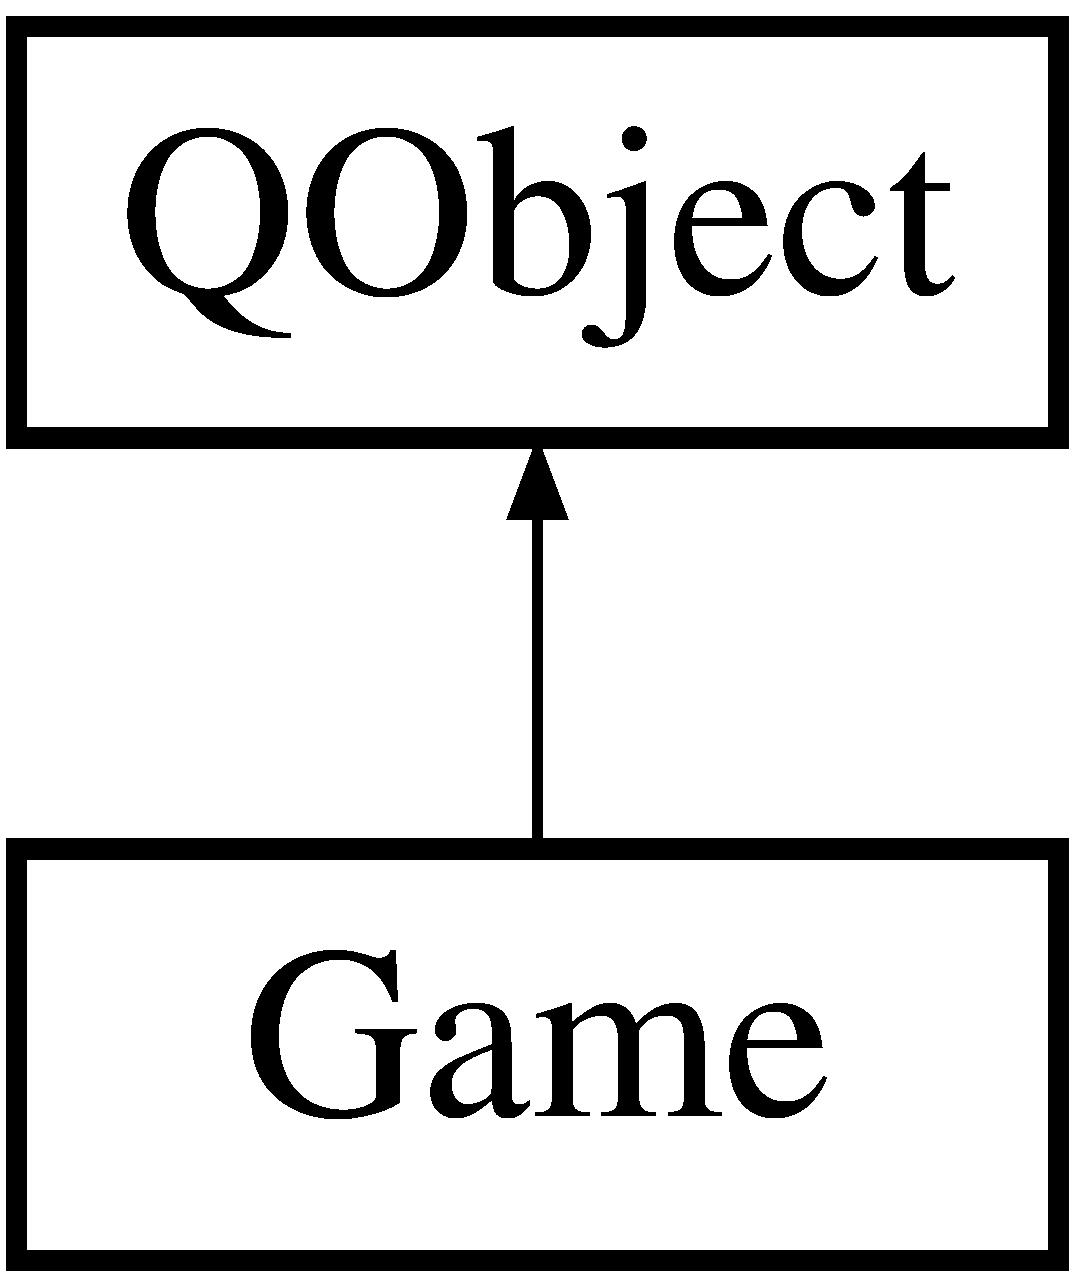
\includegraphics[height=2.000000cm]{class_game}
\end{center}
\end{figure}
\subsection*{Public Slots}
\begin{DoxyCompactItemize}
\item 
void \hyperlink{class_game_a206137b58ccb5c275619d08a9e90be37}{handle\+Cell\+Clicked} (\hyperlink{struct_board_position}{Board\+Position} where)
\item 
Q\+String \hyperlink{class_game_a5b70ad0ec696020171207825eb1915e4}{get\+Player\+Name1} ()
\item 
Q\+String \hyperlink{class_game_a03d0a6aedd4026beb2904243f0461778}{get\+Player\+Name2} ()
\item 
C\+E\+L\+L\+\_\+\+S\+T\+A\+T\+E \hyperlink{class_game_a47199b797f99bc4bbc86f286de480a5b}{get\+Players\+Token} ()
\end{DoxyCompactItemize}
\subsection*{Signals}
\begin{DoxyCompactItemize}
\item 
\hypertarget{class_game_a5d0ab94b5dca041df4288469002e56d4}{}void {\bfseries turn\+Taken} (C\+E\+L\+L\+\_\+\+S\+T\+A\+T\+E by\+Whom, C\+E\+L\+L\+\_\+\+S\+T\+A\+T\+E next\+Turn)\label{class_game_a5d0ab94b5dca041df4288469002e56d4}

\item 
\hypertarget{class_game_aaf6e4b840c1f2f3eae0fb2cbbe6ab735}{}void {\bfseries score\+Changed} (int white, int black)\label{class_game_aaf6e4b840c1f2f3eae0fb2cbbe6ab735}

\item 
\hypertarget{class_game_a9930b90b8152f151b13b5183081d76f4}{}void {\bfseries game\+Over} (C\+E\+L\+L\+\_\+\+S\+T\+A\+T\+E winner, int white, int black)\label{class_game_a9930b90b8152f151b13b5183081d76f4}

\item 
\hypertarget{class_game_a6f45946e78016e8c0bdf6abb49f39a1a}{}void {\bfseries update\+Progress} (int value)\label{class_game_a6f45946e78016e8c0bdf6abb49f39a1a}

\end{DoxyCompactItemize}
\subsection*{Public Member Functions}
\begin{DoxyCompactItemize}
\item 
\hyperlink{class_game_a01b855252c781b0d505fb1b10677e92c}{Game} (int board\+Size, int difficulty, int style, Q\+String player\+Name1, Q\+String player\+Name2)
\item 
\hyperlink{class_game_acaa1a5a4ced79038d3934dac0db2ae19}{Game} (C\+E\+L\+L\+\_\+\+S\+T\+A\+T\+E player, int board\+Size, int difficulty, int style, Q\+String player\+Name1)
\item 
\hyperlink{class_game_ae3d112ca6e0e55150d2fdbc704474530}{$\sim$\+Game} ()
\item 
Q\+Shared\+Pointer$<$ \hyperlink{class_board}{Board} $>$ \hyperlink{class_game_ab12d33e6057472bd111519b36bcf5842}{get\+Board} () const 
\end{DoxyCompactItemize}
\subsection*{Protected Member Functions}
\begin{DoxyCompactItemize}
\item 
void \hyperlink{class_game_a59cb874cb0fa9c47f4197612d9bade93}{set\+Board} (Q\+Shared\+Pointer$<$ \hyperlink{class_board}{Board} $>$ n\+Board)
\end{DoxyCompactItemize}


\subsection{Constructor \& Destructor Documentation}
\hypertarget{class_game_a01b855252c781b0d505fb1b10677e92c}{}\index{Game@{Game}!Game@{Game}}
\index{Game@{Game}!Game@{Game}}
\subsubsection[{Game}]{\setlength{\rightskip}{0pt plus 5cm}Game\+::\+Game (
\begin{DoxyParamCaption}
\item[{int}]{board\+Size, }
\item[{int}]{difficulty, }
\item[{int}]{style, }
\item[{Q\+String}]{player\+Name1, }
\item[{Q\+String}]{player\+Name2}
\end{DoxyParamCaption}
)}\label{class_game_a01b855252c781b0d505fb1b10677e92c}
Initialize a player vs player game


\begin{DoxyParams}{Parameters}
{\em board\+Size} & \\
\hline
{\em difficulty} & \\
\hline
{\em style} & \\
\hline
{\em player\+Name1} & \\
\hline
{\em player\+Name2} & \\
\hline
{\em board\+Size} & \\
\hline
{\em difficulty} & \\
\hline
{\em style} & \\
\hline
{\em player\+Name1} & \\
\hline
{\em player\+Name2} & \\
\hline
\end{DoxyParams}
\hypertarget{class_game_acaa1a5a4ced79038d3934dac0db2ae19}{}\index{Game@{Game}!Game@{Game}}
\index{Game@{Game}!Game@{Game}}
\subsubsection[{Game}]{\setlength{\rightskip}{0pt plus 5cm}Game\+::\+Game (
\begin{DoxyParamCaption}
\item[{C\+E\+L\+L\+\_\+\+S\+T\+A\+T\+E}]{player, }
\item[{int}]{board\+Size, }
\item[{int}]{difficulty, }
\item[{int}]{style, }
\item[{Q\+String}]{player\+Name1}
\end{DoxyParamCaption}
)}\label{class_game_acaa1a5a4ced79038d3934dac0db2ae19}
Initialize a player vs computer game


\begin{DoxyParams}{Parameters}
{\em player} & \\
\hline
{\em board\+Size} & \\
\hline
{\em difficulty} & \\
\hline
{\em style} & \\
\hline
{\em player\+Name1} & \\
\hline
{\em player} & \\
\hline
{\em board\+Size} & \\
\hline
{\em difficulty} & \\
\hline
{\em style} & \\
\hline
{\em player\+Name1} & \\
\hline
\end{DoxyParams}
\hypertarget{class_game_ae3d112ca6e0e55150d2fdbc704474530}{}\index{Game@{Game}!````~Game@{$\sim$\+Game}}
\index{````~Game@{$\sim$\+Game}!Game@{Game}}
\subsubsection[{$\sim$\+Game}]{\setlength{\rightskip}{0pt plus 5cm}Game\+::$\sim$\+Game (
\begin{DoxyParamCaption}
{}
\end{DoxyParamCaption}
)}\label{class_game_ae3d112ca6e0e55150d2fdbc704474530}
Destructor Removes all database connections 

\subsection{Member Function Documentation}
\hypertarget{class_game_ab12d33e6057472bd111519b36bcf5842}{}\index{Game@{Game}!get\+Board@{get\+Board}}
\index{get\+Board@{get\+Board}!Game@{Game}}
\subsubsection[{get\+Board}]{\setlength{\rightskip}{0pt plus 5cm}Q\+Shared\+Pointer$<$ {\bf Board} $>$ Game\+::get\+Board (
\begin{DoxyParamCaption}
{}
\end{DoxyParamCaption}
) const}\label{class_game_ab12d33e6057472bd111519b36bcf5842}
Gets actual reference of the board

\begin{DoxyReturn}{Returns}
Q\+Shared\+Pointer$<$\+Board$>$ 
\end{DoxyReturn}
\hypertarget{class_game_a5b70ad0ec696020171207825eb1915e4}{}\index{Game@{Game}!get\+Player\+Name1@{get\+Player\+Name1}}
\index{get\+Player\+Name1@{get\+Player\+Name1}!Game@{Game}}
\subsubsection[{get\+Player\+Name1}]{\setlength{\rightskip}{0pt plus 5cm}Q\+String Game\+::get\+Player\+Name1 (
\begin{DoxyParamCaption}
{}
\end{DoxyParamCaption}
)\hspace{0.3cm}{\ttfamily [slot]}}\label{class_game_a5b70ad0ec696020171207825eb1915e4}
Get the name of player 1

\begin{DoxyReturn}{Returns}
Q\+String 
\end{DoxyReturn}
\hypertarget{class_game_a03d0a6aedd4026beb2904243f0461778}{}\index{Game@{Game}!get\+Player\+Name2@{get\+Player\+Name2}}
\index{get\+Player\+Name2@{get\+Player\+Name2}!Game@{Game}}
\subsubsection[{get\+Player\+Name2}]{\setlength{\rightskip}{0pt plus 5cm}Q\+String Game\+::get\+Player\+Name2 (
\begin{DoxyParamCaption}
{}
\end{DoxyParamCaption}
)\hspace{0.3cm}{\ttfamily [slot]}}\label{class_game_a03d0a6aedd4026beb2904243f0461778}
Get the name of player 2

\begin{DoxyReturn}{Returns}
Q\+String 
\end{DoxyReturn}
\hypertarget{class_game_a47199b797f99bc4bbc86f286de480a5b}{}\index{Game@{Game}!get\+Players\+Token@{get\+Players\+Token}}
\index{get\+Players\+Token@{get\+Players\+Token}!Game@{Game}}
\subsubsection[{get\+Players\+Token}]{\setlength{\rightskip}{0pt plus 5cm}C\+E\+L\+L\+\_\+\+S\+T\+A\+T\+E Game\+::get\+Players\+Token (
\begin{DoxyParamCaption}
{}
\end{DoxyParamCaption}
)\hspace{0.3cm}{\ttfamily [slot]}}\label{class_game_a47199b797f99bc4bbc86f286de480a5b}
Get the token of the player (W\+H\+I\+T\+E or B\+L\+A\+C\+K) Is used in player vs computer game mode

\begin{DoxyReturn}{Returns}
C\+E\+L\+L\+\_\+\+S\+T\+A\+T\+E 
\end{DoxyReturn}
\hypertarget{class_game_a206137b58ccb5c275619d08a9e90be37}{}\index{Game@{Game}!handle\+Cell\+Clicked@{handle\+Cell\+Clicked}}
\index{handle\+Cell\+Clicked@{handle\+Cell\+Clicked}!Game@{Game}}
\subsubsection[{handle\+Cell\+Clicked}]{\setlength{\rightskip}{0pt plus 5cm}void Game\+::handle\+Cell\+Clicked (
\begin{DoxyParamCaption}
\item[{{\bf Board\+Position}}]{where}
\end{DoxyParamCaption}
)\hspace{0.3cm}{\ttfamily [slot]}}\label{class_game_a206137b58ccb5c275619d08a9e90be37}
Cell clicked event


\begin{DoxyParams}{Parameters}
{\em where} & \\
\hline
\end{DoxyParams}
\hypertarget{class_game_a59cb874cb0fa9c47f4197612d9bade93}{}\index{Game@{Game}!set\+Board@{set\+Board}}
\index{set\+Board@{set\+Board}!Game@{Game}}
\subsubsection[{set\+Board}]{\setlength{\rightskip}{0pt plus 5cm}void Game\+::set\+Board (
\begin{DoxyParamCaption}
\item[{Q\+Shared\+Pointer$<$ {\bf Board} $>$}]{n\+Board}
\end{DoxyParamCaption}
)\hspace{0.3cm}{\ttfamily [protected]}}\label{class_game_a59cb874cb0fa9c47f4197612d9bade93}
Initialize new board and connect signals / slots


\begin{DoxyParams}{Parameters}
{\em n\+Board} & \\
\hline
\end{DoxyParams}


The documentation for this class was generated from the following files\+:\begin{DoxyCompactItemize}
\item 
game.\+h\item 
game.\+cpp\end{DoxyCompactItemize}

\hypertarget{class_game_dialog}{}\section{Game\+Dialog Class Reference}
\label{class_game_dialog}\index{Game\+Dialog@{Game\+Dialog}}
Inheritance diagram for Game\+Dialog\+:\begin{figure}[H]
\begin{center}
\leavevmode
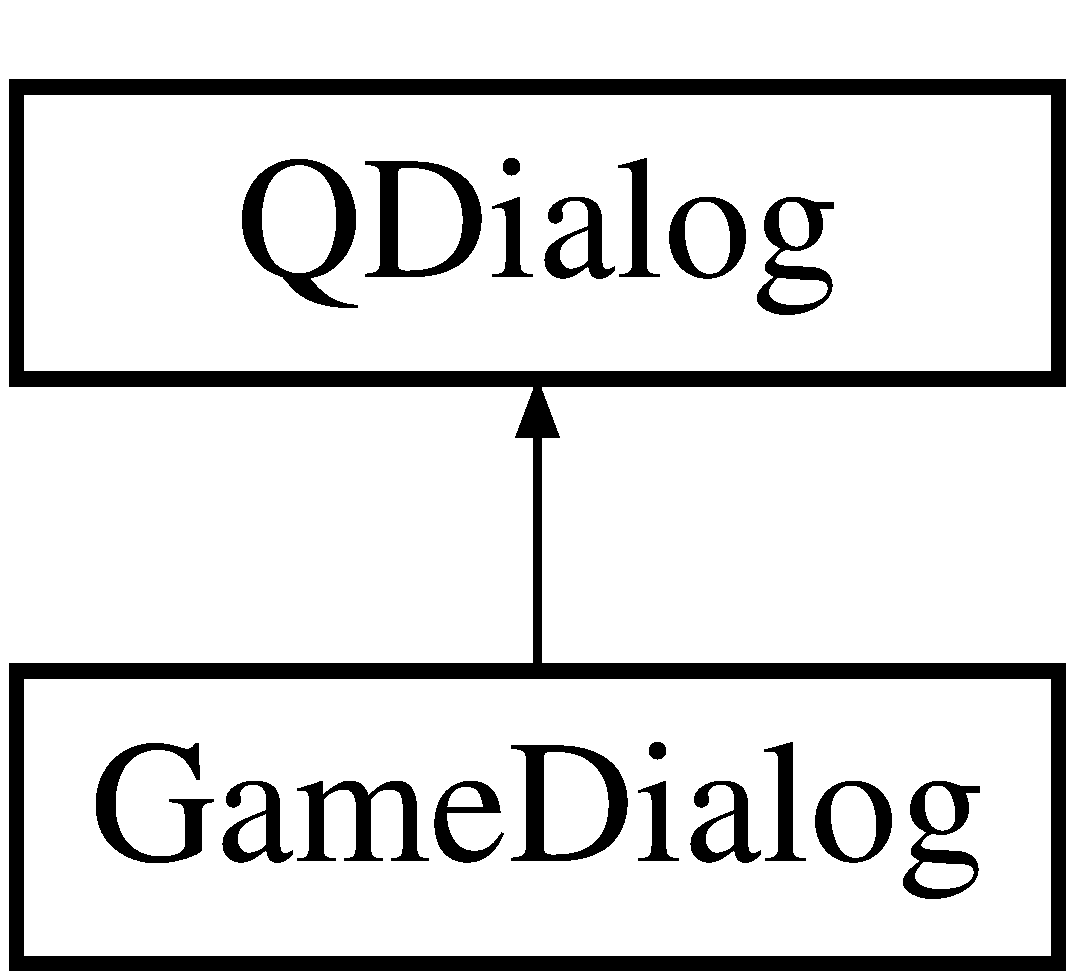
\includegraphics[height=2.000000cm]{class_game_dialog}
\end{center}
\end{figure}
\subsection*{Public Member Functions}
\begin{DoxyCompactItemize}
\item 
\hyperlink{class_game_dialog_af459e39ddd0206384ca4f125d74436af}{Game\+Dialog} (Q\+Widget $\ast$parent=0)
\item 
\hyperlink{class_game_dialog_af24640b8fb70def754b4271e9e75f56f}{$\sim$\+Game\+Dialog} ()
\item 
int \hyperlink{class_game_dialog_ad72a284a5ef97ac012b5bd4c1794264c}{get\+Difficulty} ()
\item 
int \hyperlink{class_game_dialog_a5143de940ea8144557295cd528b36359}{get\+Board\+Size} ()
\item 
C\+E\+L\+L\+\_\+\+S\+T\+A\+T\+E \hyperlink{class_game_dialog_a8a04c9b4450d66c3cffedb39fa094371}{get\+Token} ()
\item 
Q\+String \hyperlink{class_game_dialog_aeb52671e5b58aa6c1981b6d213d1e8ef}{get\+Player\+Name1} ()
\item 
Q\+String \hyperlink{class_game_dialog_ad75bffcc32e4f75b27f551a08a315c5e}{get\+Player\+Name2} ()
\item 
void \hyperlink{class_game_dialog_a6adb97b6805ed2d3e2f8c0d87e6f6812}{enable\+Player2\+Input} ()
\end{DoxyCompactItemize}


\subsection{Constructor \& Destructor Documentation}
\hypertarget{class_game_dialog_af459e39ddd0206384ca4f125d74436af}{}\index{Game\+Dialog@{Game\+Dialog}!Game\+Dialog@{Game\+Dialog}}
\index{Game\+Dialog@{Game\+Dialog}!Game\+Dialog@{Game\+Dialog}}
\subsubsection[{Game\+Dialog}]{\setlength{\rightskip}{0pt plus 5cm}Game\+Dialog\+::\+Game\+Dialog (
\begin{DoxyParamCaption}
\item[{Q\+Widget $\ast$}]{parent = {\ttfamily 0}}
\end{DoxyParamCaption}
)\hspace{0.3cm}{\ttfamily [explicit]}}\label{class_game_dialog_af459e39ddd0206384ca4f125d74436af}
Constructor


\begin{DoxyParams}{Parameters}
{\em parent} & \\
\hline
\end{DoxyParams}
\hypertarget{class_game_dialog_af24640b8fb70def754b4271e9e75f56f}{}\index{Game\+Dialog@{Game\+Dialog}!````~Game\+Dialog@{$\sim$\+Game\+Dialog}}
\index{````~Game\+Dialog@{$\sim$\+Game\+Dialog}!Game\+Dialog@{Game\+Dialog}}
\subsubsection[{$\sim$\+Game\+Dialog}]{\setlength{\rightskip}{0pt plus 5cm}Game\+Dialog\+::$\sim$\+Game\+Dialog (
\begin{DoxyParamCaption}
{}
\end{DoxyParamCaption}
)}\label{class_game_dialog_af24640b8fb70def754b4271e9e75f56f}
Destructor 

\subsection{Member Function Documentation}
\hypertarget{class_game_dialog_a6adb97b6805ed2d3e2f8c0d87e6f6812}{}\index{Game\+Dialog@{Game\+Dialog}!enable\+Player2\+Input@{enable\+Player2\+Input}}
\index{enable\+Player2\+Input@{enable\+Player2\+Input}!Game\+Dialog@{Game\+Dialog}}
\subsubsection[{enable\+Player2\+Input}]{\setlength{\rightskip}{0pt plus 5cm}void Game\+Dialog\+::enable\+Player2\+Input (
\begin{DoxyParamCaption}
{}
\end{DoxyParamCaption}
)}\label{class_game_dialog_a6adb97b6805ed2d3e2f8c0d87e6f6812}
Enables the input for a second player if the game mode is player vs player \hypertarget{class_game_dialog_a5143de940ea8144557295cd528b36359}{}\index{Game\+Dialog@{Game\+Dialog}!get\+Board\+Size@{get\+Board\+Size}}
\index{get\+Board\+Size@{get\+Board\+Size}!Game\+Dialog@{Game\+Dialog}}
\subsubsection[{get\+Board\+Size}]{\setlength{\rightskip}{0pt plus 5cm}int Game\+Dialog\+::get\+Board\+Size (
\begin{DoxyParamCaption}
{}
\end{DoxyParamCaption}
)}\label{class_game_dialog_a5143de940ea8144557295cd528b36359}
Get the configured board size

\begin{DoxyReturn}{Returns}
int 
\end{DoxyReturn}
\hypertarget{class_game_dialog_ad72a284a5ef97ac012b5bd4c1794264c}{}\index{Game\+Dialog@{Game\+Dialog}!get\+Difficulty@{get\+Difficulty}}
\index{get\+Difficulty@{get\+Difficulty}!Game\+Dialog@{Game\+Dialog}}
\subsubsection[{get\+Difficulty}]{\setlength{\rightskip}{0pt plus 5cm}int Game\+Dialog\+::get\+Difficulty (
\begin{DoxyParamCaption}
{}
\end{DoxyParamCaption}
)}\label{class_game_dialog_ad72a284a5ef97ac012b5bd4c1794264c}
Get the ai difficulty

\begin{DoxyReturn}{Returns}
int 
\end{DoxyReturn}
\hypertarget{class_game_dialog_aeb52671e5b58aa6c1981b6d213d1e8ef}{}\index{Game\+Dialog@{Game\+Dialog}!get\+Player\+Name1@{get\+Player\+Name1}}
\index{get\+Player\+Name1@{get\+Player\+Name1}!Game\+Dialog@{Game\+Dialog}}
\subsubsection[{get\+Player\+Name1}]{\setlength{\rightskip}{0pt plus 5cm}Q\+String Game\+Dialog\+::get\+Player\+Name1 (
\begin{DoxyParamCaption}
{}
\end{DoxyParamCaption}
)}\label{class_game_dialog_aeb52671e5b58aa6c1981b6d213d1e8ef}
Get the name of player 1

\begin{DoxyReturn}{Returns}
Q\+String 
\end{DoxyReturn}
\hypertarget{class_game_dialog_ad75bffcc32e4f75b27f551a08a315c5e}{}\index{Game\+Dialog@{Game\+Dialog}!get\+Player\+Name2@{get\+Player\+Name2}}
\index{get\+Player\+Name2@{get\+Player\+Name2}!Game\+Dialog@{Game\+Dialog}}
\subsubsection[{get\+Player\+Name2}]{\setlength{\rightskip}{0pt plus 5cm}Q\+String Game\+Dialog\+::get\+Player\+Name2 (
\begin{DoxyParamCaption}
{}
\end{DoxyParamCaption}
)}\label{class_game_dialog_ad75bffcc32e4f75b27f551a08a315c5e}
Get the name of player 2

\begin{DoxyReturn}{Returns}
Q\+String 
\end{DoxyReturn}
\hypertarget{class_game_dialog_a8a04c9b4450d66c3cffedb39fa094371}{}\index{Game\+Dialog@{Game\+Dialog}!get\+Token@{get\+Token}}
\index{get\+Token@{get\+Token}!Game\+Dialog@{Game\+Dialog}}
\subsubsection[{get\+Token}]{\setlength{\rightskip}{0pt plus 5cm}C\+E\+L\+L\+\_\+\+S\+T\+A\+T\+E Game\+Dialog\+::get\+Token (
\begin{DoxyParamCaption}
{}
\end{DoxyParamCaption}
)}\label{class_game_dialog_a8a04c9b4450d66c3cffedb39fa094371}
Get the token which indicates who start the game

\begin{DoxyReturn}{Returns}
C\+E\+L\+L\+\_\+\+S\+T\+A\+T\+E 
\end{DoxyReturn}


The documentation for this class was generated from the following files\+:\begin{DoxyCompactItemize}
\item 
gamedialog.\+h\item 
gamedialog.\+cpp\end{DoxyCompactItemize}

\hypertarget{class_highscore}{}\section{Highscore Class Reference}
\label{class_highscore}\index{Highscore@{Highscore}}
Inheritance diagram for Highscore\+:\begin{figure}[H]
\begin{center}
\leavevmode
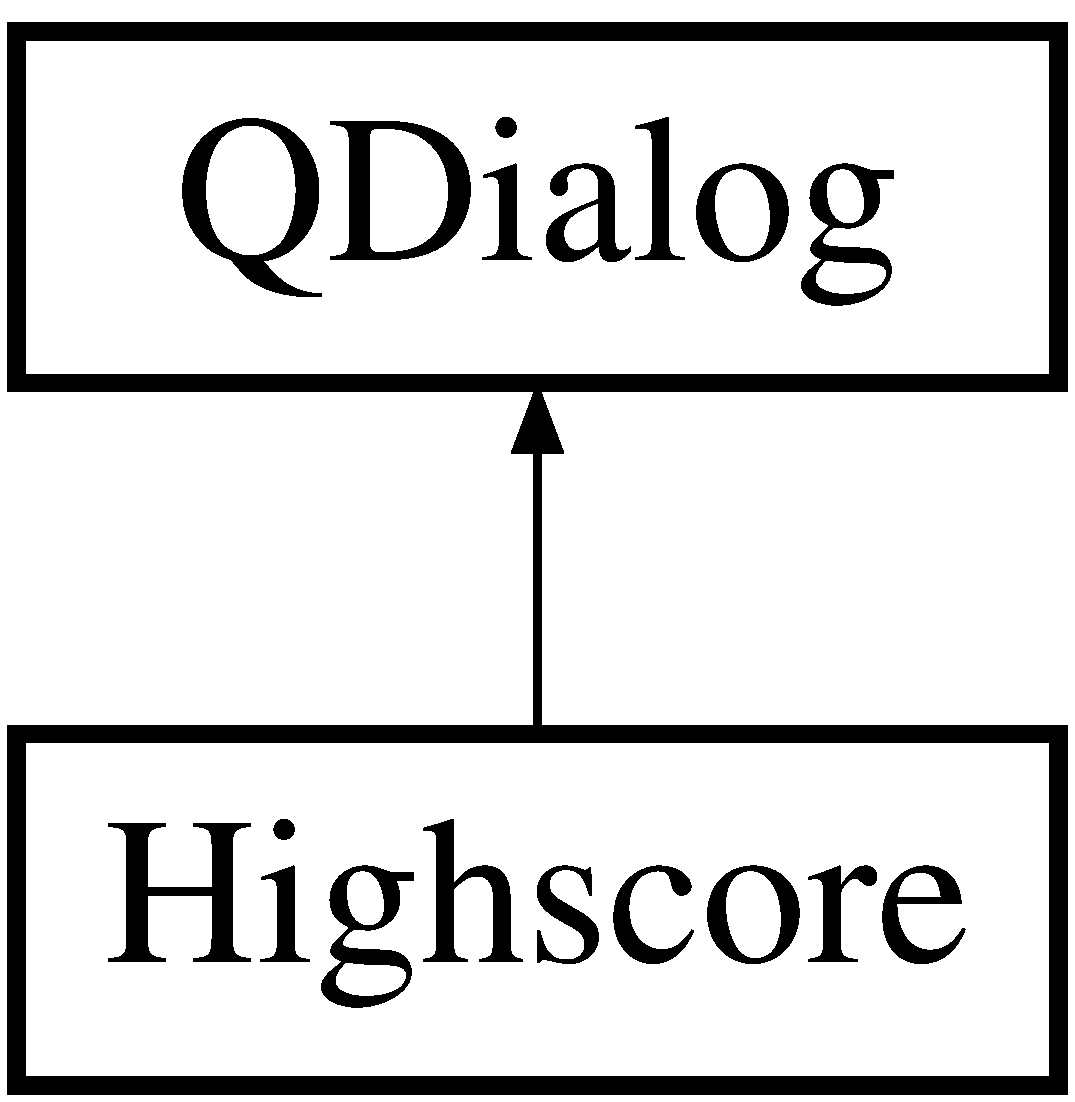
\includegraphics[height=2.000000cm]{class_highscore}
\end{center}
\end{figure}
\subsection*{Public Member Functions}
\begin{DoxyCompactItemize}
\item 
\hyperlink{class_highscore_a2b225a393a3a0e20b1ad0d42b596bcac}{Highscore} (Q\+Widget $\ast$parent=0)
\item 
\hyperlink{class_highscore_ac22dda9e0f6aeceab3c61035d6e1be5c}{$\sim$\+Highscore} ()
\end{DoxyCompactItemize}


\subsection{Constructor \& Destructor Documentation}
\hypertarget{class_highscore_a2b225a393a3a0e20b1ad0d42b596bcac}{}\index{Highscore@{Highscore}!Highscore@{Highscore}}
\index{Highscore@{Highscore}!Highscore@{Highscore}}
\subsubsection[{Highscore}]{\setlength{\rightskip}{0pt plus 5cm}Highscore\+::\+Highscore (
\begin{DoxyParamCaption}
\item[{Q\+Widget $\ast$}]{parent = {\ttfamily 0}}
\end{DoxyParamCaption}
)\hspace{0.3cm}{\ttfamily [explicit]}}\label{class_highscore_a2b225a393a3a0e20b1ad0d42b596bcac}
Constructor


\begin{DoxyParams}{Parameters}
{\em parent} & \\
\hline
\end{DoxyParams}
\hypertarget{class_highscore_ac22dda9e0f6aeceab3c61035d6e1be5c}{}\index{Highscore@{Highscore}!````~Highscore@{$\sim$\+Highscore}}
\index{````~Highscore@{$\sim$\+Highscore}!Highscore@{Highscore}}
\subsubsection[{$\sim$\+Highscore}]{\setlength{\rightskip}{0pt plus 5cm}Highscore\+::$\sim$\+Highscore (
\begin{DoxyParamCaption}
{}
\end{DoxyParamCaption}
)}\label{class_highscore_ac22dda9e0f6aeceab3c61035d6e1be5c}
Destructor Removes all database connections 

The documentation for this class was generated from the following files\+:\begin{DoxyCompactItemize}
\item 
highscore.\+h\item 
highscore.\+cpp\end{DoxyCompactItemize}

\hypertarget{class_main_window}{}\section{Main\+Window Class Reference}
\label{class_main_window}\index{Main\+Window@{Main\+Window}}
Inheritance diagram for Main\+Window\+:\begin{figure}[H]
\begin{center}
\leavevmode
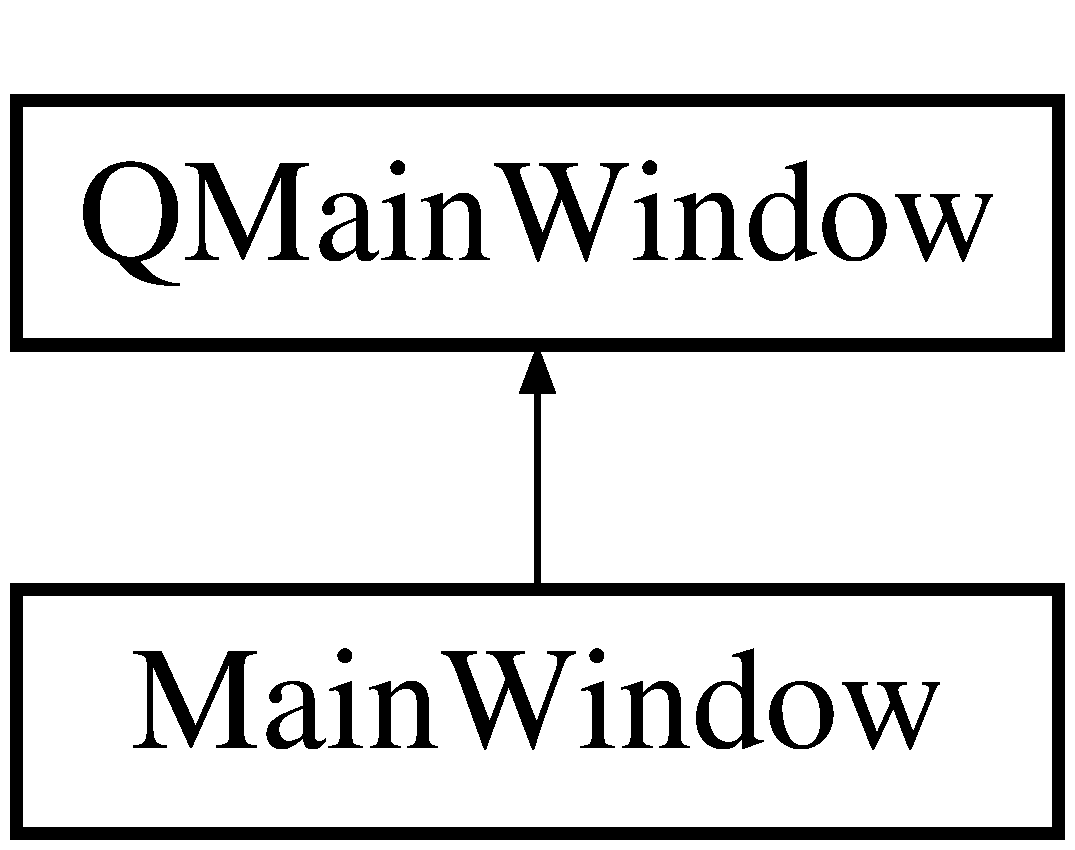
\includegraphics[height=2.000000cm]{class_main_window}
\end{center}
\end{figure}
\subsection*{Public Member Functions}
\begin{DoxyCompactItemize}
\item 
\hyperlink{class_main_window_a8b244be8b7b7db1b08de2a2acb9409db}{Main\+Window} (Q\+Widget $\ast$parent=0)
\item 
\hyperlink{class_main_window_ae98d00a93bc118200eeef9f9bba1dba7}{$\sim$\+Main\+Window} ()
\end{DoxyCompactItemize}
\subsection*{Protected Member Functions}
\begin{DoxyCompactItemize}
\item 
void \hyperlink{class_main_window_af4ca5d0d3d18ddcb7d54b6596bbf4797}{change\+Event} (Q\+Event $\ast$e)
\end{DoxyCompactItemize}


\subsection{Constructor \& Destructor Documentation}
\hypertarget{class_main_window_a8b244be8b7b7db1b08de2a2acb9409db}{}\index{Main\+Window@{Main\+Window}!Main\+Window@{Main\+Window}}
\index{Main\+Window@{Main\+Window}!Main\+Window@{Main\+Window}}
\subsubsection[{Main\+Window}]{\setlength{\rightskip}{0pt plus 5cm}Main\+Window\+::\+Main\+Window (
\begin{DoxyParamCaption}
\item[{Q\+Widget $\ast$}]{parent = {\ttfamily 0}}
\end{DoxyParamCaption}
)\hspace{0.3cm}{\ttfamily [explicit]}}\label{class_main_window_a8b244be8b7b7db1b08de2a2acb9409db}
Constructor


\begin{DoxyParams}{Parameters}
{\em parent} & \\
\hline
\end{DoxyParams}
\hypertarget{class_main_window_ae98d00a93bc118200eeef9f9bba1dba7}{}\index{Main\+Window@{Main\+Window}!````~Main\+Window@{$\sim$\+Main\+Window}}
\index{````~Main\+Window@{$\sim$\+Main\+Window}!Main\+Window@{Main\+Window}}
\subsubsection[{$\sim$\+Main\+Window}]{\setlength{\rightskip}{0pt plus 5cm}Main\+Window\+::$\sim$\+Main\+Window (
\begin{DoxyParamCaption}
{}
\end{DoxyParamCaption}
)}\label{class_main_window_ae98d00a93bc118200eeef9f9bba1dba7}
Destructor 

\subsection{Member Function Documentation}
\hypertarget{class_main_window_af4ca5d0d3d18ddcb7d54b6596bbf4797}{}\index{Main\+Window@{Main\+Window}!change\+Event@{change\+Event}}
\index{change\+Event@{change\+Event}!Main\+Window@{Main\+Window}}
\subsubsection[{change\+Event}]{\setlength{\rightskip}{0pt plus 5cm}void Main\+Window\+::change\+Event (
\begin{DoxyParamCaption}
\item[{Q\+Event $\ast$}]{event}
\end{DoxyParamCaption}
)\hspace{0.3cm}{\ttfamily [protected]}}\label{class_main_window_af4ca5d0d3d18ddcb7d54b6596bbf4797}
Change event (need for runtime translation but doesn\textquotesingle{}t work atm)


\begin{DoxyParams}{Parameters}
{\em event} & \\
\hline
\end{DoxyParams}


The documentation for this class was generated from the following files\+:\begin{DoxyCompactItemize}
\item 
mainwindow.\+h\item 
mainwindow.\+cpp\end{DoxyCompactItemize}

\hypertarget{class_minimax}{}\section{Minimax Class Reference}
\label{class_minimax}\index{Minimax@{Minimax}}
Inheritance diagram for Minimax\+:\begin{figure}[H]
\begin{center}
\leavevmode
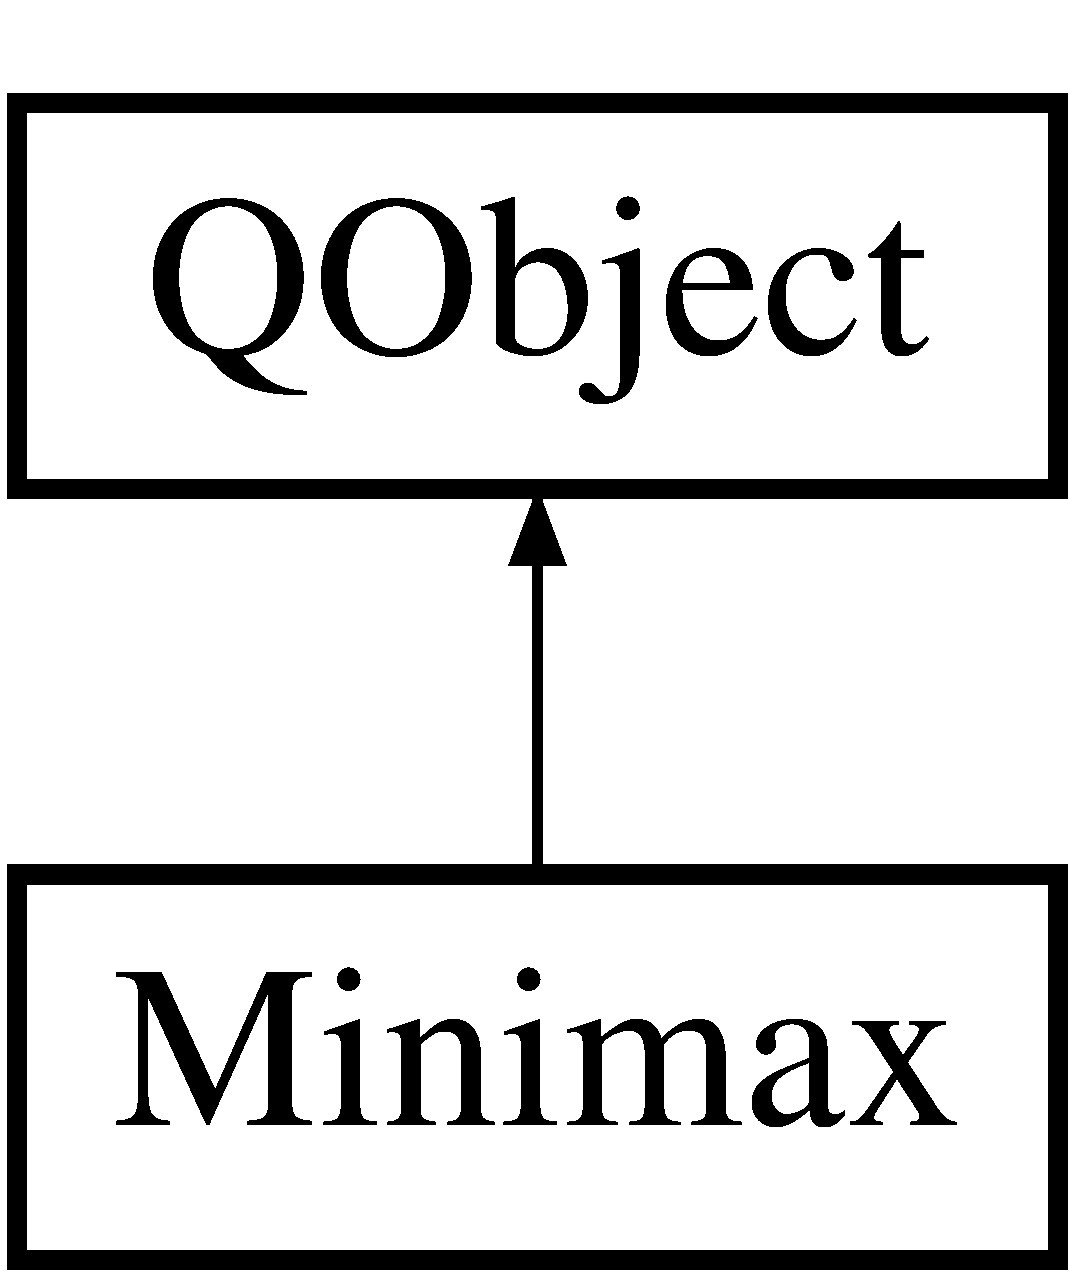
\includegraphics[height=2.000000cm]{class_minimax}
\end{center}
\end{figure}
\subsection*{Signals}
\begin{DoxyCompactItemize}
\item 
\hypertarget{class_minimax_a7562b56f3c805f0732cd04ff575a649b}{}void {\bfseries update\+Progress} (int value)\label{class_minimax_a7562b56f3c805f0732cd04ff575a649b}

\end{DoxyCompactItemize}
\subsection*{Public Member Functions}
\begin{DoxyCompactItemize}
\item 
\hyperlink{class_minimax_a9d2f91d5a6a7b582d095f1ff30454754}{Minimax} (Q\+Shared\+Pointer$<$ \hyperlink{class_board}{Board} $>$ root\+Node, int max\+Depth)
\item 
virtual \hyperlink{class_minimax_ac88b5b70cb204684d2a33bbc5e815d9a}{$\sim$\+Minimax} ()
\item 
int \hyperlink{class_minimax_a73a16d428768b37ac6377d4450acfb48}{search} ()
\item 
\hyperlink{struct_board_position}{Board\+Position} \hyperlink{class_minimax_ab78e32e5568d4f023775aa55d2f0b613}{get\+Best\+Move} () const 
\end{DoxyCompactItemize}


\subsection{Constructor \& Destructor Documentation}
\hypertarget{class_minimax_a9d2f91d5a6a7b582d095f1ff30454754}{}\index{Minimax@{Minimax}!Minimax@{Minimax}}
\index{Minimax@{Minimax}!Minimax@{Minimax}}
\subsubsection[{Minimax}]{\setlength{\rightskip}{0pt plus 5cm}Minimax\+::\+Minimax (
\begin{DoxyParamCaption}
\item[{Q\+Shared\+Pointer$<$ {\bf Board} $>$}]{root\+Node, }
\item[{int}]{max\+Depth}
\end{DoxyParamCaption}
)}\label{class_minimax_a9d2f91d5a6a7b582d095f1ff30454754}
Constructor


\begin{DoxyParams}{Parameters}
{\em root\+Node} & \\
\hline
{\em max\+Depth} & \\
\hline
\end{DoxyParams}
\hypertarget{class_minimax_ac88b5b70cb204684d2a33bbc5e815d9a}{}\index{Minimax@{Minimax}!````~Minimax@{$\sim$\+Minimax}}
\index{````~Minimax@{$\sim$\+Minimax}!Minimax@{Minimax}}
\subsubsection[{$\sim$\+Minimax}]{\setlength{\rightskip}{0pt plus 5cm}Minimax\+::$\sim$\+Minimax (
\begin{DoxyParamCaption}
{}
\end{DoxyParamCaption}
)\hspace{0.3cm}{\ttfamily [virtual]}}\label{class_minimax_ac88b5b70cb204684d2a33bbc5e815d9a}
Desctructor 

\subsection{Member Function Documentation}
\hypertarget{class_minimax_ab78e32e5568d4f023775aa55d2f0b613}{}\index{Minimax@{Minimax}!get\+Best\+Move@{get\+Best\+Move}}
\index{get\+Best\+Move@{get\+Best\+Move}!Minimax@{Minimax}}
\subsubsection[{get\+Best\+Move}]{\setlength{\rightskip}{0pt plus 5cm}{\bf Board\+Position} Minimax\+::get\+Best\+Move (
\begin{DoxyParamCaption}
{}
\end{DoxyParamCaption}
) const}\label{class_minimax_ab78e32e5568d4f023775aa55d2f0b613}
Just a getter to get the last calculated best move because the algorithm is too heavy to recalculate every single time

\begin{DoxyReturn}{Returns}
\hyperlink{struct_board_position}{Board\+Position} 
\end{DoxyReturn}
\hypertarget{class_minimax_a73a16d428768b37ac6377d4450acfb48}{}\index{Minimax@{Minimax}!search@{search}}
\index{search@{search}!Minimax@{Minimax}}
\subsubsection[{search}]{\setlength{\rightskip}{0pt plus 5cm}int Minimax\+::search (
\begin{DoxyParamCaption}
{}
\end{DoxyParamCaption}
)}\label{class_minimax_a73a16d428768b37ac6377d4450acfb48}
Search the tree Begins at the root node

\begin{DoxyReturn}{Returns}
int 
\end{DoxyReturn}


The documentation for this class was generated from the following files\+:\begin{DoxyCompactItemize}
\item 
minimax.\+h\item 
minimax.\+cpp\end{DoxyCompactItemize}

\hypertarget{struct_settings_dialog_1_1_settings}{}\section{Settings\+Dialog\+:\+:Settings Struct Reference}
\label{struct_settings_dialog_1_1_settings}\index{Settings\+Dialog\+::\+Settings@{Settings\+Dialog\+::\+Settings}}
\subsection*{Public Attributes}
\begin{DoxyCompactItemize}
\item 
\hypertarget{struct_settings_dialog_1_1_settings_a5f026eb24c2e78595c4e67ef5bd137c0}{}int {\bfseries style}\label{struct_settings_dialog_1_1_settings_a5f026eb24c2e78595c4e67ef5bd137c0}

\item 
\hypertarget{struct_settings_dialog_1_1_settings_af4430b9479a649af088e985f8e7d7c27}{}int {\bfseries language}\label{struct_settings_dialog_1_1_settings_af4430b9479a649af088e985f8e7d7c27}

\end{DoxyCompactItemize}


The documentation for this struct was generated from the following file\+:\begin{DoxyCompactItemize}
\item 
settingsdialog.\+h\end{DoxyCompactItemize}

\hypertarget{struct_ui_1_1_settings}{}\section{Ui\+:\+:Settings Struct Reference}
\label{struct_ui_1_1_settings}\index{Ui\+::\+Settings@{Ui\+::\+Settings}}
\subsection*{Public Attributes}
\begin{DoxyCompactItemize}
\item 
\hypertarget{struct_ui_1_1_settings_a88c0666d27a688b854313d4e8be84ce4}{}int {\bfseries difficulty} = 1\label{struct_ui_1_1_settings_a88c0666d27a688b854313d4e8be84ce4}

\item 
\hypertarget{struct_ui_1_1_settings_aa322f139c01a4a7bb2cb803d53d11702}{}int {\bfseries board\+Size} = 8\label{struct_ui_1_1_settings_aa322f139c01a4a7bb2cb803d53d11702}

\end{DoxyCompactItemize}


The documentation for this struct was generated from the following file\+:\begin{DoxyCompactItemize}
\item 
gamedialog.\+h\end{DoxyCompactItemize}

\hypertarget{class_settings_dialog}{}\section{Settings\+Dialog Class Reference}
\label{class_settings_dialog}\index{Settings\+Dialog@{Settings\+Dialog}}
Inheritance diagram for Settings\+Dialog\+:\begin{figure}[H]
\begin{center}
\leavevmode
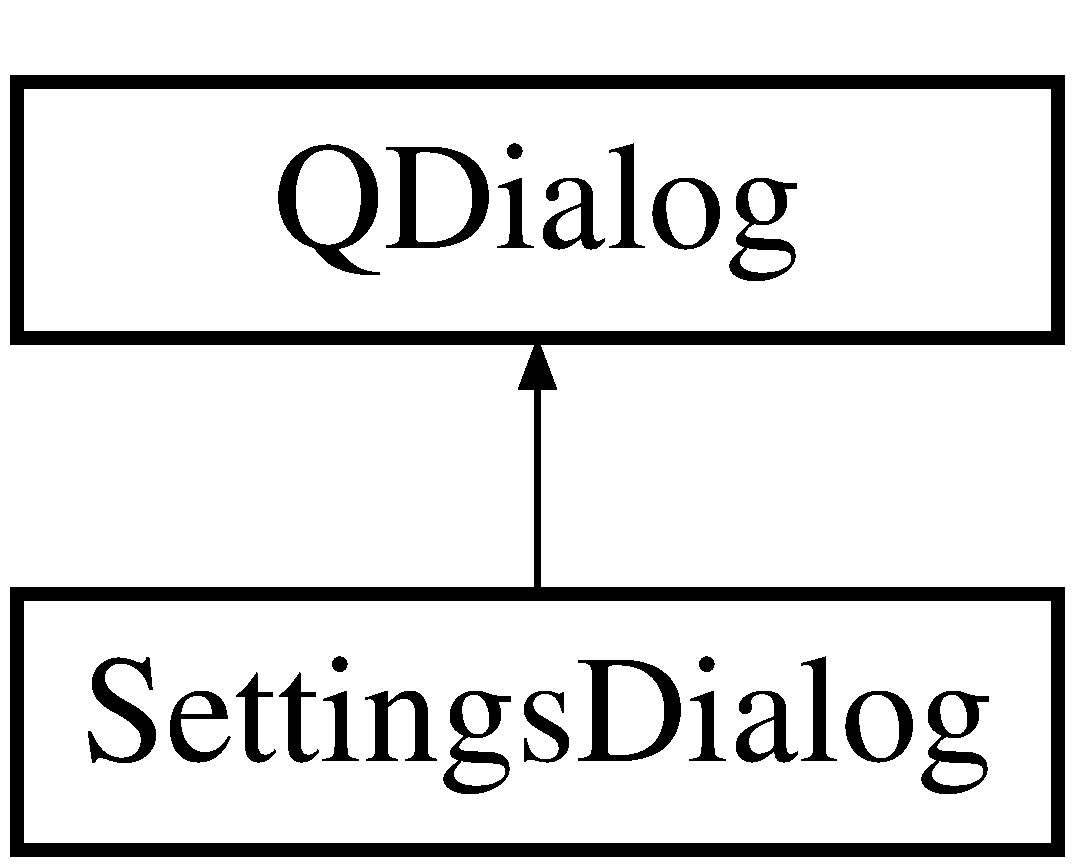
\includegraphics[height=2.000000cm]{class_settings_dialog}
\end{center}
\end{figure}
\subsection*{Classes}
\begin{DoxyCompactItemize}
\item 
struct \hyperlink{struct_settings_dialog_1_1_settings}{Settings}
\end{DoxyCompactItemize}
\subsection*{Public Member Functions}
\begin{DoxyCompactItemize}
\item 
\hyperlink{class_settings_dialog_a9933956b777b2c0451e9119581cc22fb}{Settings\+Dialog} (Q\+Widget $\ast$parent=0)
\item 
\hyperlink{class_settings_dialog_ac48f54d4472902be0a3845a69167f068}{$\sim$\+Settings\+Dialog} ()
\item 
\hyperlink{struct_settings_dialog_1_1_settings}{Settings} \hyperlink{class_settings_dialog_afeb533d711d0392b9856c63b40b65ad7}{settings} () const 
\item 
int \hyperlink{class_settings_dialog_a67d4687c793b02da6dba1d2cd9bf701c}{get\+Language} ()
\item 
int \hyperlink{class_settings_dialog_a9162f4376c8e3889dabd281428c87337}{get\+Style} ()
\end{DoxyCompactItemize}
\subsection*{Protected Member Functions}
\begin{DoxyCompactItemize}
\item 
void \hyperlink{class_settings_dialog_a0d0670544a7d571840aa54fb4b74aed7}{change\+Event} (Q\+Event $\ast$e)
\end{DoxyCompactItemize}


\subsection{Constructor \& Destructor Documentation}
\hypertarget{class_settings_dialog_a9933956b777b2c0451e9119581cc22fb}{}\index{Settings\+Dialog@{Settings\+Dialog}!Settings\+Dialog@{Settings\+Dialog}}
\index{Settings\+Dialog@{Settings\+Dialog}!Settings\+Dialog@{Settings\+Dialog}}
\subsubsection[{Settings\+Dialog}]{\setlength{\rightskip}{0pt plus 5cm}Settings\+Dialog\+::\+Settings\+Dialog (
\begin{DoxyParamCaption}
\item[{Q\+Widget $\ast$}]{parent = {\ttfamily 0}}
\end{DoxyParamCaption}
)\hspace{0.3cm}{\ttfamily [explicit]}}\label{class_settings_dialog_a9933956b777b2c0451e9119581cc22fb}
Constructor Loads all settings from ini


\begin{DoxyParams}{Parameters}
{\em parent} & \\
\hline
\end{DoxyParams}
\hypertarget{class_settings_dialog_ac48f54d4472902be0a3845a69167f068}{}\index{Settings\+Dialog@{Settings\+Dialog}!````~Settings\+Dialog@{$\sim$\+Settings\+Dialog}}
\index{````~Settings\+Dialog@{$\sim$\+Settings\+Dialog}!Settings\+Dialog@{Settings\+Dialog}}
\subsubsection[{$\sim$\+Settings\+Dialog}]{\setlength{\rightskip}{0pt plus 5cm}Settings\+Dialog\+::$\sim$\+Settings\+Dialog (
\begin{DoxyParamCaption}
{}
\end{DoxyParamCaption}
)}\label{class_settings_dialog_ac48f54d4472902be0a3845a69167f068}
Destructor Saves all settings to ini 

\subsection{Member Function Documentation}
\hypertarget{class_settings_dialog_a0d0670544a7d571840aa54fb4b74aed7}{}\index{Settings\+Dialog@{Settings\+Dialog}!change\+Event@{change\+Event}}
\index{change\+Event@{change\+Event}!Settings\+Dialog@{Settings\+Dialog}}
\subsubsection[{change\+Event}]{\setlength{\rightskip}{0pt plus 5cm}void Settings\+Dialog\+::change\+Event (
\begin{DoxyParamCaption}
\item[{Q\+Event $\ast$}]{event}
\end{DoxyParamCaption}
)\hspace{0.3cm}{\ttfamily [protected]}}\label{class_settings_dialog_a0d0670544a7d571840aa54fb4b74aed7}
Change event (need for runtime translation but doesn\textquotesingle{}t work atm)


\begin{DoxyParams}{Parameters}
{\em event} & \\
\hline
\end{DoxyParams}
\hypertarget{class_settings_dialog_a67d4687c793b02da6dba1d2cd9bf701c}{}\index{Settings\+Dialog@{Settings\+Dialog}!get\+Language@{get\+Language}}
\index{get\+Language@{get\+Language}!Settings\+Dialog@{Settings\+Dialog}}
\subsubsection[{get\+Language}]{\setlength{\rightskip}{0pt plus 5cm}int Settings\+Dialog\+::get\+Language (
\begin{DoxyParamCaption}
{}
\end{DoxyParamCaption}
)}\label{class_settings_dialog_a67d4687c793b02da6dba1d2cd9bf701c}
Get the actual language from ini

\begin{DoxyReturn}{Returns}
int 
\end{DoxyReturn}
\hypertarget{class_settings_dialog_a9162f4376c8e3889dabd281428c87337}{}\index{Settings\+Dialog@{Settings\+Dialog}!get\+Style@{get\+Style}}
\index{get\+Style@{get\+Style}!Settings\+Dialog@{Settings\+Dialog}}
\subsubsection[{get\+Style}]{\setlength{\rightskip}{0pt plus 5cm}int Settings\+Dialog\+::get\+Style (
\begin{DoxyParamCaption}
{}
\end{DoxyParamCaption}
)}\label{class_settings_dialog_a9162f4376c8e3889dabd281428c87337}
Get the actual style from ini

\begin{DoxyReturn}{Returns}
int 
\end{DoxyReturn}
\hypertarget{class_settings_dialog_afeb533d711d0392b9856c63b40b65ad7}{}\index{Settings\+Dialog@{Settings\+Dialog}!settings@{settings}}
\index{settings@{settings}!Settings\+Dialog@{Settings\+Dialog}}
\subsubsection[{settings}]{\setlength{\rightskip}{0pt plus 5cm}{\bf Settings\+Dialog\+::\+Settings} Settings\+Dialog\+::settings (
\begin{DoxyParamCaption}
{}
\end{DoxyParamCaption}
) const}\label{class_settings_dialog_afeb533d711d0392b9856c63b40b65ad7}
Get the actual settings

\begin{DoxyReturn}{Returns}
\hyperlink{struct_settings_dialog_1_1_settings}{Settings\+Dialog\+::\+Settings} 
\end{DoxyReturn}


The documentation for this class was generated from the following files\+:\begin{DoxyCompactItemize}
\item 
settingsdialog.\+h\item 
settingsdialog.\+cpp\end{DoxyCompactItemize}

\hypertarget{class_test}{}\section{Test$<$ T $>$ Class Template Reference}
\label{class_test}\index{Test$<$ T $>$@{Test$<$ T $>$}}
\subsection*{Public Member Functions}
\begin{DoxyCompactItemize}
\item 
\hypertarget{class_test_a744fa6648f5397560c203dc145146787}{}{\bfseries Test} (const Q\+String \&name)\label{class_test_a744fa6648f5397560c203dc145146787}

\end{DoxyCompactItemize}
\subsection*{Public Attributes}
\begin{DoxyCompactItemize}
\item 
\hypertarget{class_test_acfb1db9d3c0e3f372aa716b6ead5a00c}{}Q\+Shared\+Pointer$<$ T $>$ {\bfseries child}\label{class_test_acfb1db9d3c0e3f372aa716b6ead5a00c}

\end{DoxyCompactItemize}


The documentation for this class was generated from the following file\+:\begin{DoxyCompactItemize}
\item 
Auto\+Test.\+h\end{DoxyCompactItemize}

%--- End generated contents ---

% Index
\backmatter
\newpage
\phantomsection
\clearemptydoublepage
\addcontentsline{toc}{chapter}{Index}
\printindex

\end{document}
